
\documentclass[]{article}
\usepackage[utf8]{inputenc}
\usepackage[usenames,dvipsnames]{xcolor}
\usepackage{fullpage}
\usepackage[upright]{fourier}
\usepackage{tkz-graph}
\usepackage{fancyhdr}
\usetikzlibrary{arrows}
\begin{document}

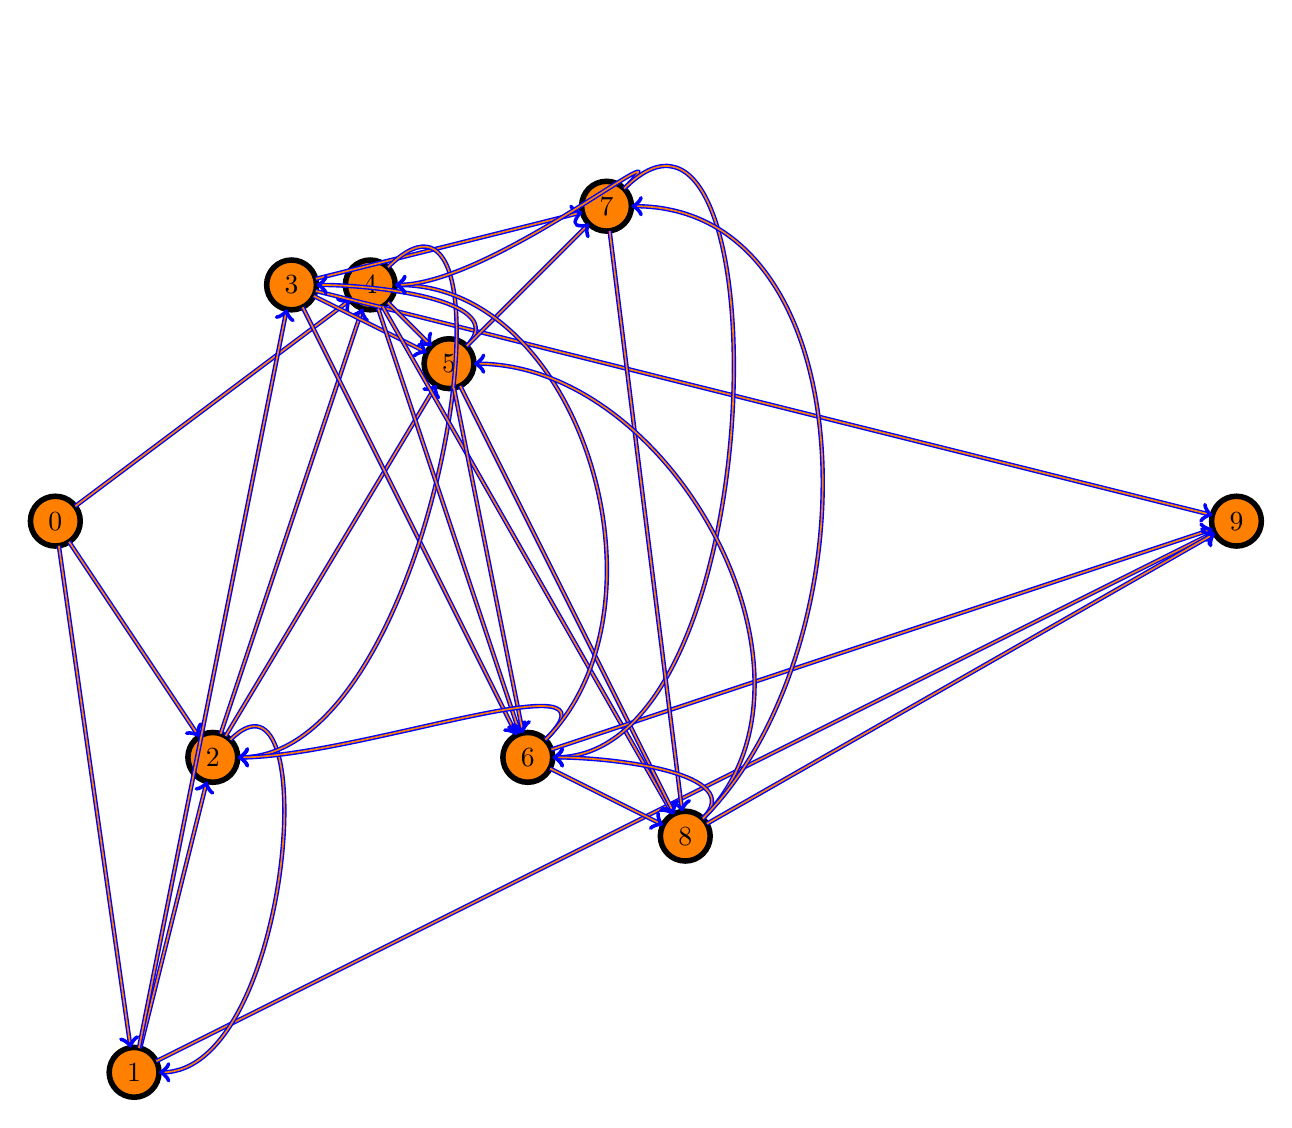
\begin{tikzpicture}
\SetVertexNormal[Shape      = circle,
FillColor  = orange,
LineWidth  = 2pt]
\SetUpEdge[lw         = 0.5pt,
color      = black,
labelcolor = white,
labeltext  = red,
labelstyle = {sloped,text=blue}]
\tikzstyle{TempStyle}=[double = orange]
\Vertex[x=-10, y=8]{0}
\Vertex[x=-9, y=1]{1}
\Vertex[x=-8, y=5]{2}
\Vertex[x=-7, y=11]{3}
\Vertex[x=-6, y=11]{4}
\Vertex[x=-5, y=10]{5}
\Vertex[x=-4, y=5]{6}
\Vertex[x=-3, y=12]{7}
\Vertex[x=-2, y=4]{8}
\Vertex[x=5, y=8]{9}
\tikzset{EdgeStyle/.style={->,TempStyle,relative=false,right=60,color=blue}}
\Edge(0)(1)
\tikzset{EdgeStyle/.style={->,TempStyle,relative=false,right=60,color=blue}}
\Edge(0)(2)
\tikzset{EdgeStyle/.style={->,TempStyle,relative=false,right=60,color=blue}}
\Edge(0)(4)
\tikzset{EdgeStyle/.style={->,TempStyle,relative=false,right=60,color=blue}}
\Edge(1)(2)
\tikzset{EdgeStyle/.style={->,TempStyle,relative=false,right=60,color=blue}}
\Edge(1)(3)
\tikzset{EdgeStyle/.style={->,TempStyle,relative=false,right=60,color=blue}}
\Edge(1)(9)
\tikzset{EdgeStyle/.style={->,TempStyle,relative=false,left=60,color=blue,in=0,draw}}
\Edge(2)(1)
\tikzset{EdgeStyle/.style={->,TempStyle,relative=false,right=60,color=blue}}
\Edge(2)(4)
\tikzset{EdgeStyle/.style={->,TempStyle,relative=false,right=60,color=blue}}
\Edge(2)(5)
\tikzset{EdgeStyle/.style={->,TempStyle,relative=false,right=60,color=blue}}
\Edge(3)(5)
\tikzset{EdgeStyle/.style={->,TempStyle,relative=false,right=60,color=blue}}
\Edge(3)(6)
\tikzset{EdgeStyle/.style={->,TempStyle,relative=false,right=60,color=blue}}
\Edge(3)(7)
\tikzset{EdgeStyle/.style={->,TempStyle,relative=false,right=60,color=blue}}
\Edge(3)(9)
\tikzset{EdgeStyle/.style={->,TempStyle,relative=false,left=60,color=blue,in=0,draw}}
\Edge(4)(2)
\tikzset{EdgeStyle/.style={->,TempStyle,relative=false,right=60,color=blue}}
\Edge(4)(5)
\tikzset{EdgeStyle/.style={->,TempStyle,relative=false,right=60,color=blue}}
\Edge(4)(6)
\tikzset{EdgeStyle/.style={->,TempStyle,relative=false,right=60,color=blue}}
\Edge(4)(8)
\tikzset{EdgeStyle/.style={->,TempStyle,relative=false,left=60,color=blue,in=0,draw}}
\Edge(5)(3)
\tikzset{EdgeStyle/.style={->,TempStyle,relative=false,right=60,color=blue}}
\Edge(5)(6)
\tikzset{EdgeStyle/.style={->,TempStyle,relative=false,right=60,color=blue}}
\Edge(5)(7)
\tikzset{EdgeStyle/.style={->,TempStyle,relative=false,right=60,color=blue}}
\Edge(5)(8)
\tikzset{EdgeStyle/.style={->,TempStyle,relative=false,left=60,color=blue,in=0,draw}}
\Edge(6)(2)
\tikzset{EdgeStyle/.style={->,TempStyle,relative=false,left=60,color=blue,in=0,draw}}
\Edge(6)(4)
\tikzset{EdgeStyle/.style={->,TempStyle,relative=false,right=60,color=blue}}
\Edge(6)(8)
\tikzset{EdgeStyle/.style={->,TempStyle,relative=false,right=60,color=blue}}
\Edge(6)(9)
\tikzset{EdgeStyle/.style={->,TempStyle,relative=false,left=60,color=blue,in=0,draw}}
\Edge(7)(4)
\tikzset{EdgeStyle/.style={->,TempStyle,relative=false,left=60,color=blue,in=0,draw}}
\Edge(7)(6)
\tikzset{EdgeStyle/.style={->,TempStyle,relative=false,right=60,color=blue}}
\Edge(7)(8)
\tikzset{EdgeStyle/.style={->,TempStyle,relative=false,left=60,color=blue,in=0,draw}}
\Edge(8)(5)
\tikzset{EdgeStyle/.style={->,TempStyle,relative=false,left=60,color=blue,in=0,draw}}
\Edge(8)(6)
\tikzset{EdgeStyle/.style={->,TempStyle,relative=false,left=60,color=blue,in=0,draw}}
\Edge(8)(7)
\tikzset{EdgeStyle/.style={->,TempStyle,relative=false,right=60,color=blue}}
\Edge(8)(9)
\end{tikzpicture}\\
\begin{center}\begin{tabular}{l c}\\
\textcolor{orange}{\LARGE$\rightarrow$} & Chemin \\
 \textcolor{red}{\LARGE$\rightarrow$} & Créations arcs\\
 \textcolor{green}{\LARGE$\rightarrow$} & Modification flot\\
\end{tabular}
\end{center}
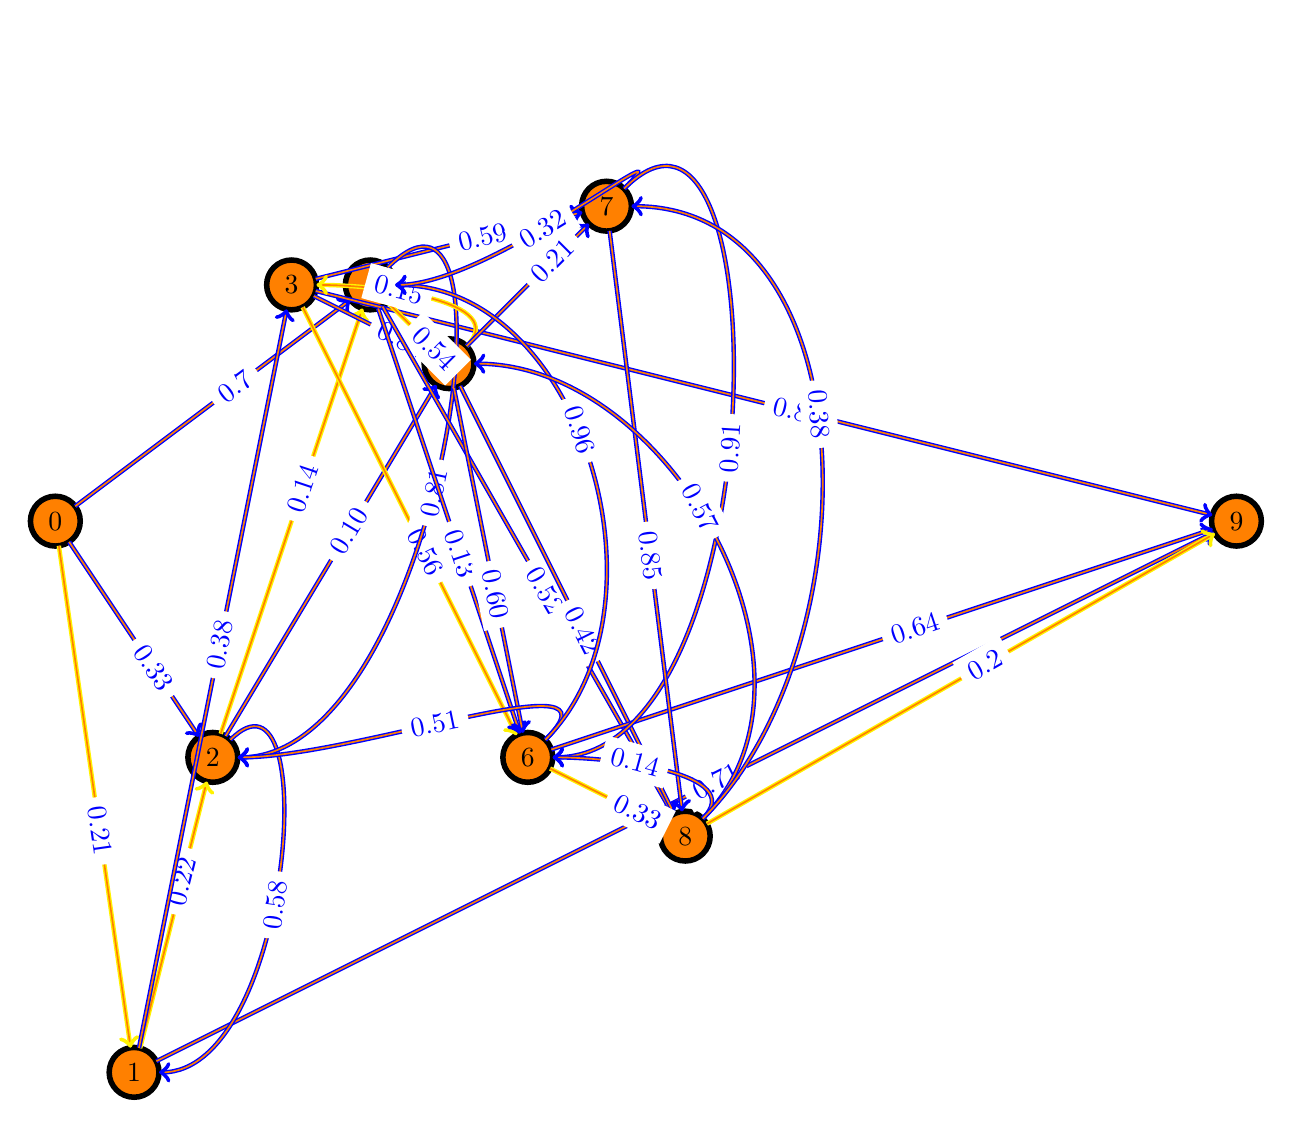
\begin{tikzpicture}
\SetVertexNormal[Shape      = circle,
FillColor  = orange,
LineWidth  = 2pt]
\SetUpEdge[lw         = 0.5pt,
color      = black,
labelcolor = white,
labeltext  = red,
labelstyle = {sloped,text=blue}]
\tikzstyle{TempStyle}=[double = orange]
\Vertex[x=-10, y=8]{0}
\Vertex[x=-9, y=1]{1}
\Vertex[x=-8, y=5]{2}
\Vertex[x=-7, y=11]{3}
\Vertex[x=-6, y=11]{4}
\Vertex[x=-5, y=10]{5}
\Vertex[x=-4, y=5]{6}
\Vertex[x=-3, y=12]{7}
\Vertex[x=-2, y=4]{8}
\Vertex[x=5, y=8]{9}
\tikzset{EdgeStyle/.style={->,TempStyle,relative=false,right=60,color=yellow}}
\Edge[label=$0.21$](0)(1)
\tikzset{EdgeStyle/.style={->,TempStyle,relative=false,right=60,color=blue}}
\Edge[label=$0.33$](0)(2)
\tikzset{EdgeStyle/.style={->,TempStyle,relative=false,right=60,color=blue}}
\Edge[label=$0.7$](0)(4)
\tikzset{EdgeStyle/.style={->,TempStyle,relative=false,right=60,color=yellow}}
\Edge[label=$0.22$](1)(2)
\tikzset{EdgeStyle/.style={->,TempStyle,relative=false,right=60,color=blue}}
\Edge[label=$0.38$](1)(3)
\tikzset{EdgeStyle/.style={->,TempStyle,relative=false,right=60,color=blue}}
\Edge[label=$0.71$](1)(9)
\tikzset{EdgeStyle/.style={->,TempStyle,relative=false,left=60,color=blue,in=0,draw}}
\Edge[label=$0.58$](2)(1)
\tikzset{EdgeStyle/.style={->,TempStyle,relative=false,right=60,color=yellow}}
\Edge[label=$0.14$](2)(4)
\tikzset{EdgeStyle/.style={->,TempStyle,relative=false,right=60,color=blue}}
\Edge[label=$0.10$](2)(5)
\tikzset{EdgeStyle/.style={->,TempStyle,relative=false,right=60,color=blue}}
\Edge[label=$0.8$](3)(5)
\tikzset{EdgeStyle/.style={->,TempStyle,relative=false,right=60,color=yellow}}
\Edge[label=$0.56$](3)(6)
\tikzset{EdgeStyle/.style={->,TempStyle,relative=false,right=60,color=blue}}
\Edge[label=$0.59$](3)(7)
\tikzset{EdgeStyle/.style={->,TempStyle,relative=false,right=60,color=blue}}
\Edge[label=$0.8$](3)(9)
\tikzset{EdgeStyle/.style={->,TempStyle,relative=false,left=60,color=blue,in=0,draw}}
\Edge[label=$0.81$](4)(2)
\tikzset{EdgeStyle/.style={->,TempStyle,relative=false,right=60,color=yellow}}
\Edge[label=$0.54$](4)(5)
\tikzset{EdgeStyle/.style={->,TempStyle,relative=false,right=60,color=blue}}
\Edge[label=$0.13$](4)(6)
\tikzset{EdgeStyle/.style={->,TempStyle,relative=false,right=60,color=blue}}
\Edge[label=$0.52$](4)(8)
\tikzset{EdgeStyle/.style={->,TempStyle,relative=false,left=60,in=0,color=yellow}}
\Edge[label=$0.15$](5)(3)
\tikzset{EdgeStyle/.style={->,TempStyle,relative=false,right=60,color=blue}}
\Edge[label=$0.60$](5)(6)
\tikzset{EdgeStyle/.style={->,TempStyle,relative=false,right=60,color=blue}}
\Edge[label=$0.21$](5)(7)
\tikzset{EdgeStyle/.style={->,TempStyle,relative=false,right=60,color=blue}}
\Edge[label=$0.42$](5)(8)
\tikzset{EdgeStyle/.style={->,TempStyle,relative=false,left=60,color=blue,in=0,draw}}
\Edge[label=$0.51$](6)(2)
\tikzset{EdgeStyle/.style={->,TempStyle,relative=false,left=60,color=blue,in=0,draw}}
\Edge[label=$0.96$](6)(4)
\tikzset{EdgeStyle/.style={->,TempStyle,relative=false,right=60,color=yellow}}
\Edge[label=$0.33$](6)(8)
\tikzset{EdgeStyle/.style={->,TempStyle,relative=false,right=60,color=blue}}
\Edge[label=$0.64$](6)(9)
\tikzset{EdgeStyle/.style={->,TempStyle,relative=false,left=60,color=blue,in=0,draw}}
\Edge[label=$0.32$](7)(4)
\tikzset{EdgeStyle/.style={->,TempStyle,relative=false,left=60,color=blue,in=0,draw}}
\Edge[label=$0.91$](7)(6)
\tikzset{EdgeStyle/.style={->,TempStyle,relative=false,right=60,color=blue}}
\Edge[label=$0.85$](7)(8)
\tikzset{EdgeStyle/.style={->,TempStyle,relative=false,left=60,color=blue,in=0,draw}}
\Edge[label=$0.57$](8)(5)
\tikzset{EdgeStyle/.style={->,TempStyle,relative=false,left=60,color=blue,in=0,draw}}
\Edge[label=$0.14$](8)(6)
\tikzset{EdgeStyle/.style={->,TempStyle,relative=false,left=60,color=blue,in=0,draw}}
\Edge[label=$0.38$](8)(7)
\tikzset{EdgeStyle/.style={->,TempStyle,relative=false,right=60,color=yellow}}
\Edge[label=$0.2$](8)(9)
\end{tikzpicture}\\
\begin{center}\begin{tabular}{l c}\\
\textcolor{orange}{\LARGE$\rightarrow$} & Chemin \\
 \textcolor{red}{\LARGE$\rightarrow$} & Créations arcs\\
 \textcolor{green}{\LARGE$\rightarrow$} & Modification flot\\
\end{tabular}
\end{center}
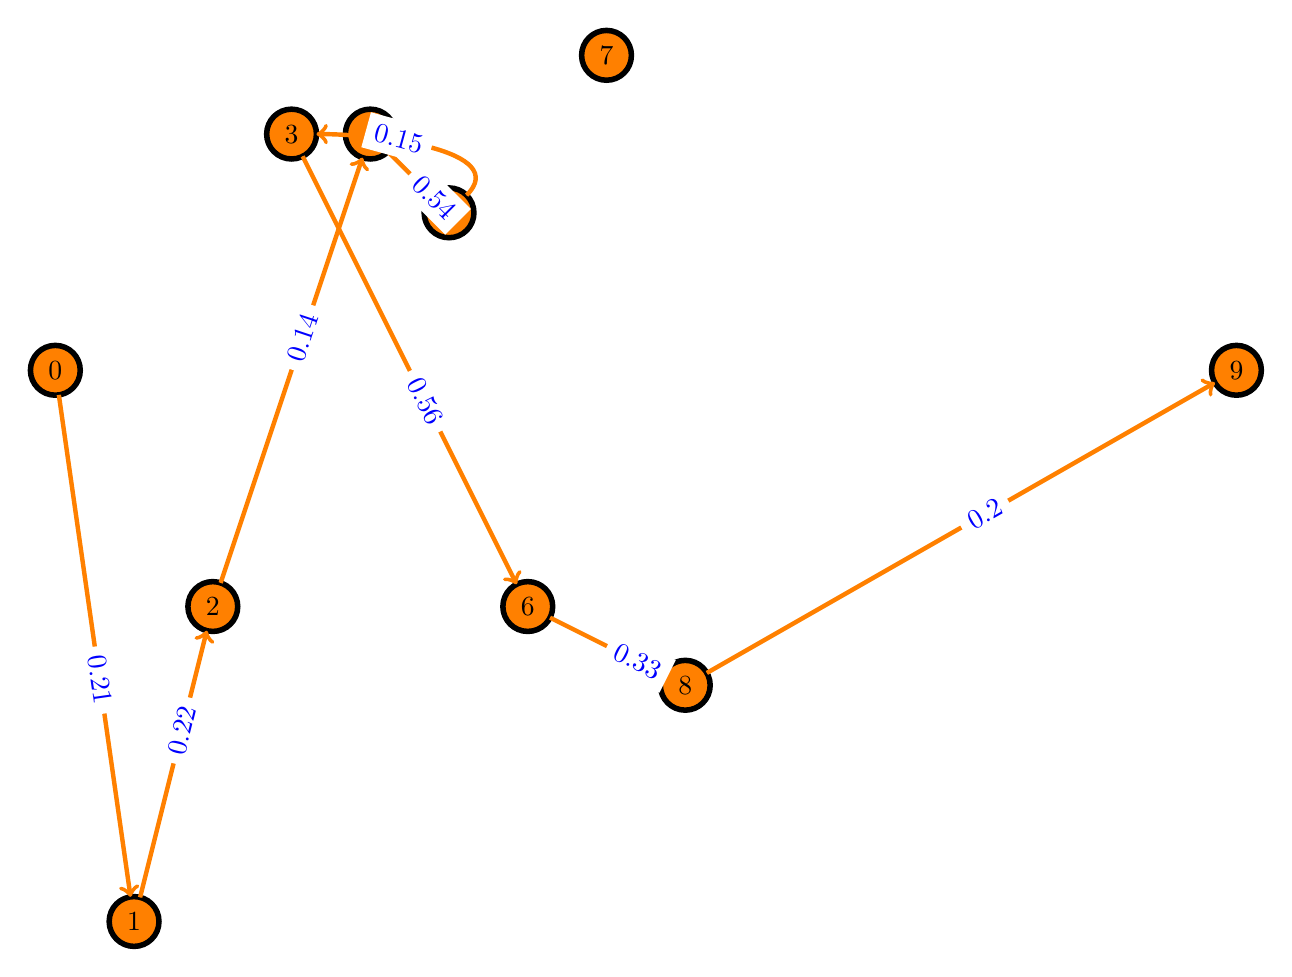
\begin{tikzpicture}
\SetVertexNormal[Shape      = circle,
FillColor  = orange,
LineWidth  = 2pt]
\SetUpEdge[lw         = 0.5pt,
color      = black,
labelcolor = white,
labeltext  = red,
labelstyle = {sloped,text=blue}]
\tikzstyle{TempStyle}=[double = orange]
\Vertex[x=-10, y=8]{0}
\Vertex[x=-9, y=1]{1}
\Vertex[x=-8, y=5]{2}
\Vertex[x=-7, y=11]{3}
\Vertex[x=-6, y=11]{4}
\Vertex[x=-5, y=10]{5}
\Vertex[x=-4, y=5]{6}
\Vertex[x=-3, y=12]{7}
\Vertex[x=-2, y=4]{8}
\Vertex[x=5, y=8]{9}
\tikzset{EdgeStyle/.style={->,TempStyle,relative=false,right=60,color=orange}}
\Edge[label=$0.21$](0)(1)
\tikzset{EdgeStyle/.style={->,TempStyle,relative=false,right=60,color=orange}}
\Edge[label=$0.22$](1)(2)
\tikzset{EdgeStyle/.style={->,TempStyle,relative=false,right=60,color=orange}}
\Edge[label=$0.14$](2)(4)
\tikzset{EdgeStyle/.style={->,TempStyle,relative=false,right=60,color=orange}}
\Edge[label=$0.56$](3)(6)
\tikzset{EdgeStyle/.style={->,TempStyle,relative=false,right=60,color=orange}}
\Edge[label=$0.54$](4)(5)
\tikzset{EdgeStyle/.style={->,TempStyle,relative=false,left=60,color=orange,in=0,draw}}
\Edge[label=$0.15$](5)(3)
\tikzset{EdgeStyle/.style={->,TempStyle,relative=false,right=60,color=orange}}
\Edge[label=$0.33$](6)(8)
\tikzset{EdgeStyle/.style={->,TempStyle,relative=false,right=60,color=orange}}
\Edge[label=$0.2$](8)(9)
\end{tikzpicture}\\
\begin{center}\begin{tabular}{l c}\\
\textcolor{orange}{\LARGE$\rightarrow$} & Chemin \\
 \textcolor{red}{\LARGE$\rightarrow$} & Créations arcs\\
 \textcolor{green}{\LARGE$\rightarrow$} & Modification flot\\
\end{tabular}
\end{center}
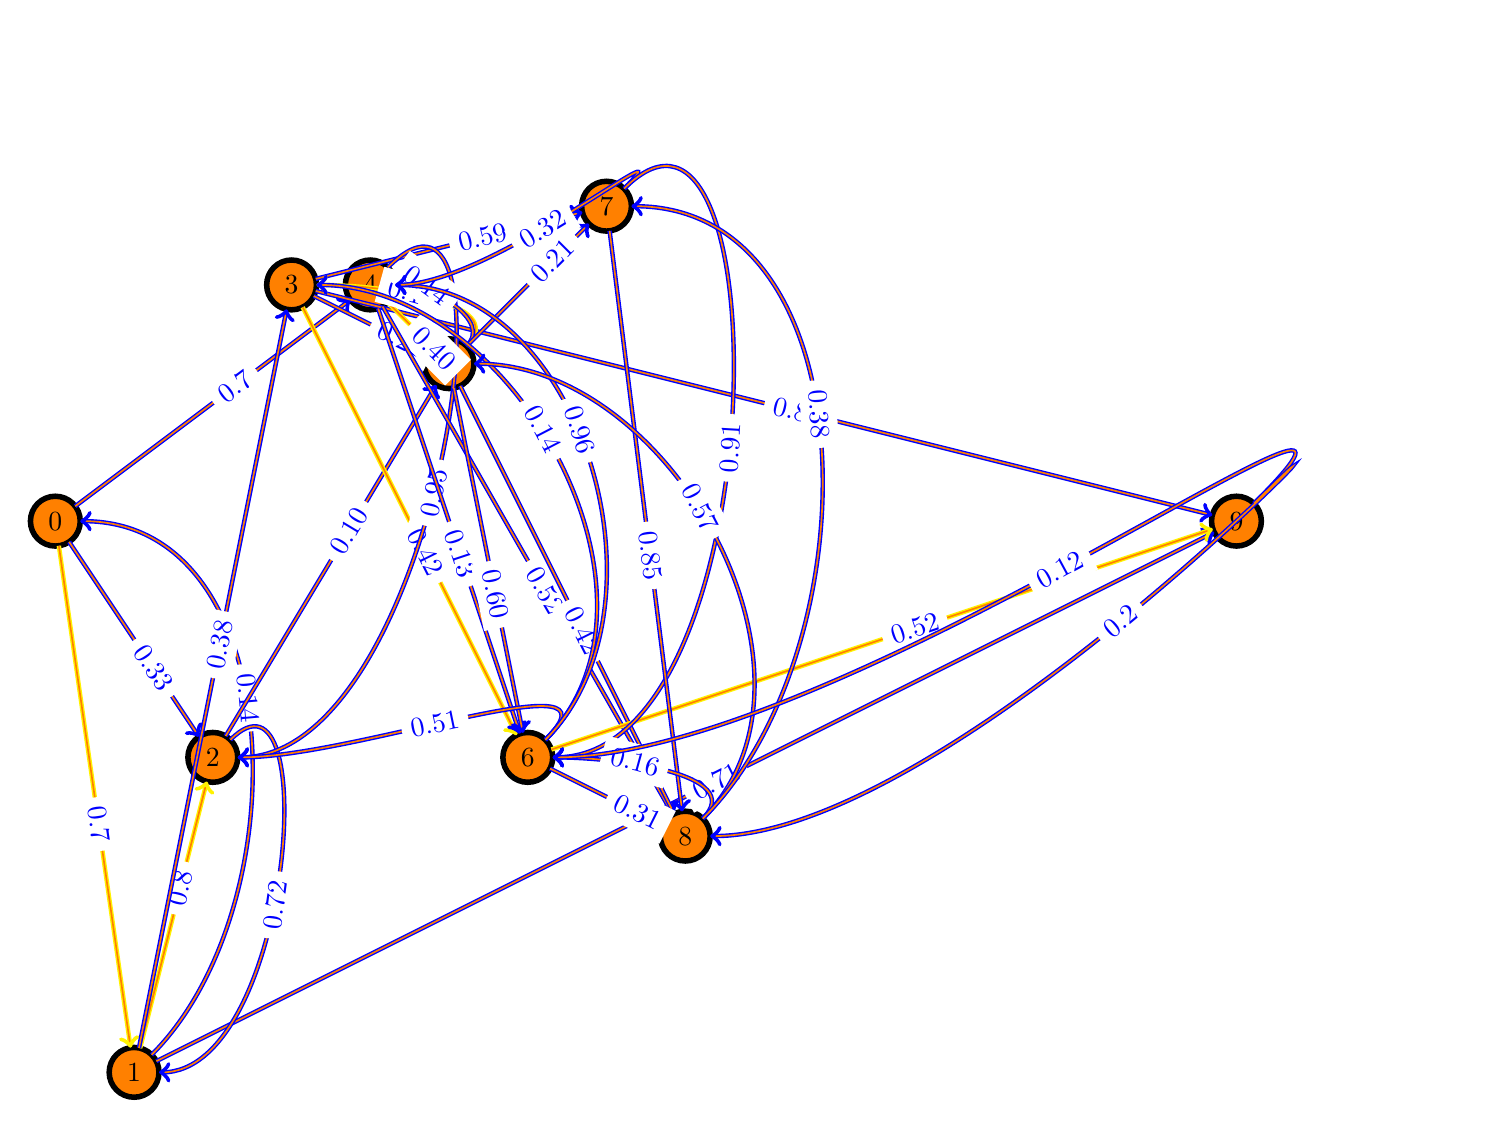
\begin{tikzpicture}
\SetVertexNormal[Shape      = circle,
FillColor  = orange,
LineWidth  = 2pt]
\SetUpEdge[lw         = 0.5pt,
color      = black,
labelcolor = white,
labeltext  = red,
labelstyle = {sloped,text=blue}]
\tikzstyle{TempStyle}=[double = orange]
\Vertex[x=-10, y=8]{0}
\Vertex[x=-9, y=1]{1}
\Vertex[x=-8, y=5]{2}
\Vertex[x=-7, y=11]{3}
\Vertex[x=-6, y=11]{4}
\Vertex[x=-5, y=10]{5}
\Vertex[x=-4, y=5]{6}
\Vertex[x=-3, y=12]{7}
\Vertex[x=-2, y=4]{8}
\Vertex[x=5, y=8]{9}
\tikzset{EdgeStyle/.style={->,TempStyle,relative=false,right=60,color=yellow}}
\Edge[label=$0.7$](0)(1)
\tikzset{EdgeStyle/.style={->,TempStyle,relative=false,right=60,color=blue}}
\Edge[label=$0.33$](0)(2)
\tikzset{EdgeStyle/.style={->,TempStyle,relative=false,right=60,color=blue}}
\Edge[label=$0.7$](0)(4)
\tikzset{EdgeStyle/.style={->,TempStyle,relative=false,left=60,color=blue,in=0,draw}}
\Edge[label=$0.14$](1)(0)
\tikzset{EdgeStyle/.style={->,TempStyle,relative=false,right=60,color=yellow}}
\Edge[label=$0.8$](1)(2)
\tikzset{EdgeStyle/.style={->,TempStyle,relative=false,right=60,color=blue}}
\Edge[label=$0.38$](1)(3)
\tikzset{EdgeStyle/.style={->,TempStyle,relative=false,right=60,color=blue}}
\Edge[label=$0.71$](1)(9)
\tikzset{EdgeStyle/.style={->,TempStyle,relative=false,left=60,color=blue,in=0,draw}}
\Edge[label=$0.72$](2)(1)
\tikzset{EdgeStyle/.style={->,TempStyle,relative=false,right=60,color=blue}}
\Edge[label=$0.10$](2)(5)
\tikzset{EdgeStyle/.style={->,TempStyle,relative=false,right=60,color=blue}}
\Edge[label=$0.22$](3)(5)
\tikzset{EdgeStyle/.style={->,TempStyle,relative=false,right=60,color=yellow}}
\Edge[label=$0.42$](3)(6)
\tikzset{EdgeStyle/.style={->,TempStyle,relative=false,right=60,color=blue}}
\Edge[label=$0.59$](3)(7)
\tikzset{EdgeStyle/.style={->,TempStyle,relative=false,right=60,color=blue}}
\Edge[label=$0.8$](3)(9)
\tikzset{EdgeStyle/.style={->,TempStyle,relative=false,left=60,color=blue,in=0,draw}}
\Edge[label=$0.95$](4)(2)
\tikzset{EdgeStyle/.style={->,TempStyle,relative=false,right=60,color=yellow}}
\Edge[label=$0.40$](4)(5)
\tikzset{EdgeStyle/.style={->,TempStyle,relative=false,right=60,color=blue}}
\Edge[label=$0.13$](4)(6)
\tikzset{EdgeStyle/.style={->,TempStyle,relative=false,right=60,color=blue}}
\Edge[label=$0.52$](4)(8)
\tikzset{EdgeStyle/.style={->,TempStyle,relative=false,left=60,in=0,color=yellow}}
\Edge[label=$0.1$](5)(3)
\tikzset{EdgeStyle/.style={->,TempStyle,relative=false,left=60,color=blue,in=0,draw}}
\Edge[label=$0.14$](5)(4)
\tikzset{EdgeStyle/.style={->,TempStyle,relative=false,right=60,color=blue}}
\Edge[label=$0.60$](5)(6)
\tikzset{EdgeStyle/.style={->,TempStyle,relative=false,right=60,color=blue}}
\Edge[label=$0.21$](5)(7)
\tikzset{EdgeStyle/.style={->,TempStyle,relative=false,right=60,color=blue}}
\Edge[label=$0.42$](5)(8)
\tikzset{EdgeStyle/.style={->,TempStyle,relative=false,left=60,color=blue,in=0,draw}}
\Edge[label=$0.51$](6)(2)
\tikzset{EdgeStyle/.style={->,TempStyle,relative=false,left=60,color=blue,in=0,draw}}
\Edge[label=$0.14$](6)(3)
\tikzset{EdgeStyle/.style={->,TempStyle,relative=false,left=60,color=blue,in=0,draw}}
\Edge[label=$0.96$](6)(4)
\tikzset{EdgeStyle/.style={->,TempStyle,relative=false,right=60,color=blue}}
\Edge[label=$0.31$](6)(8)
\tikzset{EdgeStyle/.style={->,TempStyle,relative=false,right=60,color=yellow}}
\Edge[label=$0.52$](6)(9)
\tikzset{EdgeStyle/.style={->,TempStyle,relative=false,left=60,color=blue,in=0,draw}}
\Edge[label=$0.32$](7)(4)
\tikzset{EdgeStyle/.style={->,TempStyle,relative=false,left=60,color=blue,in=0,draw}}
\Edge[label=$0.91$](7)(6)
\tikzset{EdgeStyle/.style={->,TempStyle,relative=false,right=60,color=blue}}
\Edge[label=$0.85$](7)(8)
\tikzset{EdgeStyle/.style={->,TempStyle,relative=false,left=60,color=blue,in=0,draw}}
\Edge[label=$0.57$](8)(5)
\tikzset{EdgeStyle/.style={->,TempStyle,relative=false,left=60,color=blue,in=0,draw}}
\Edge[label=$0.16$](8)(6)
\tikzset{EdgeStyle/.style={->,TempStyle,relative=false,left=60,color=blue,in=0,draw}}
\Edge[label=$0.38$](8)(7)
\tikzset{EdgeStyle/.style={->,TempStyle,relative=false,left=60,color=blue,in=0,draw}}
\Edge[label=$0.12$](9)(6)
\tikzset{EdgeStyle/.style={->,TempStyle,relative=false,left=60,color=blue,in=0,draw}}
\Edge[label=$0.2$](9)(8)
\end{tikzpicture}\\
\begin{center}\begin{tabular}{l c}\\
\textcolor{orange}{\LARGE$\rightarrow$} & Chemin \\
 \textcolor{red}{\LARGE$\rightarrow$} & Créations arcs\\
 \textcolor{green}{\LARGE$\rightarrow$} & Modification flot\\
\end{tabular}
\end{center}
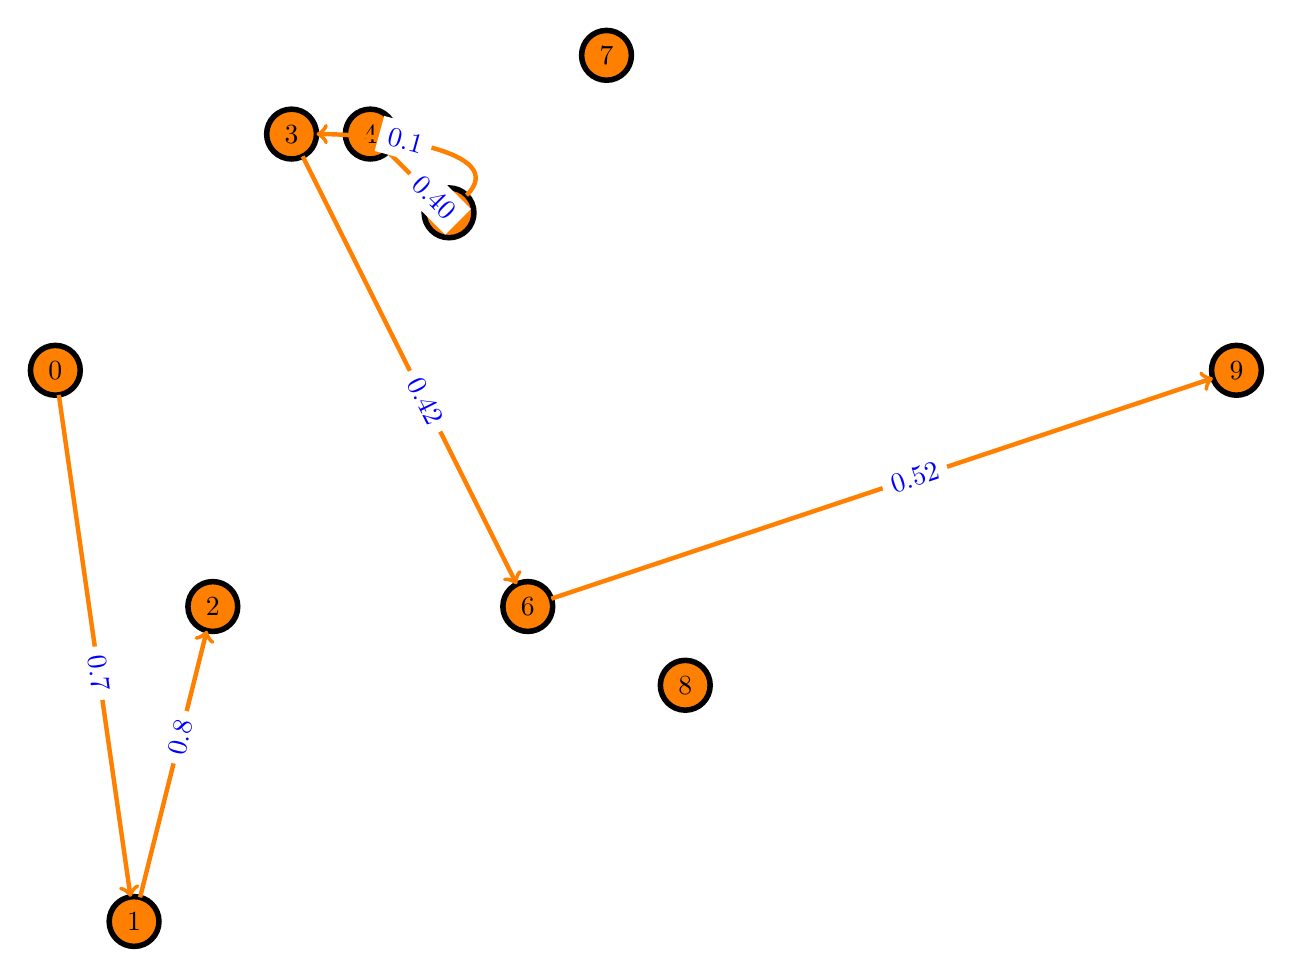
\begin{tikzpicture}
\SetVertexNormal[Shape      = circle,
FillColor  = orange,
LineWidth  = 2pt]
\SetUpEdge[lw         = 0.5pt,
color      = black,
labelcolor = white,
labeltext  = red,
labelstyle = {sloped,text=blue}]
\tikzstyle{TempStyle}=[double = orange]
\Vertex[x=-10, y=8]{0}
\Vertex[x=-9, y=1]{1}
\Vertex[x=-8, y=5]{2}
\Vertex[x=-7, y=11]{3}
\Vertex[x=-6, y=11]{4}
\Vertex[x=-5, y=10]{5}
\Vertex[x=-4, y=5]{6}
\Vertex[x=-3, y=12]{7}
\Vertex[x=-2, y=4]{8}
\Vertex[x=5, y=8]{9}
\tikzset{EdgeStyle/.style={->,TempStyle,relative=false,right=60,color=orange}}
\Edge[label=$0.7$](0)(1)
\tikzset{EdgeStyle/.style={->,TempStyle,relative=false,right=60,color=orange}}
\Edge[label=$0.8$](1)(2)
\tikzset{EdgeStyle/.style={->,TempStyle,relative=false,right=60,color=orange}}
\Edge[label=$0.42$](3)(6)
\tikzset{EdgeStyle/.style={->,TempStyle,relative=false,right=60,color=orange}}
\Edge[label=$0.40$](4)(5)
\tikzset{EdgeStyle/.style={->,TempStyle,relative=false,left=60,color=orange,in=0,draw}}
\Edge[label=$0.1$](5)(3)
\tikzset{EdgeStyle/.style={->,TempStyle,relative=false,right=60,color=orange}}
\Edge[label=$0.52$](6)(9)
\end{tikzpicture}\\
\begin{center}\begin{tabular}{l c}\\
\textcolor{orange}{\LARGE$\rightarrow$} & Chemin \\
 \textcolor{red}{\LARGE$\rightarrow$} & Créations arcs\\
 \textcolor{green}{\LARGE$\rightarrow$} & Modification flot\\
\end{tabular}
\end{center}
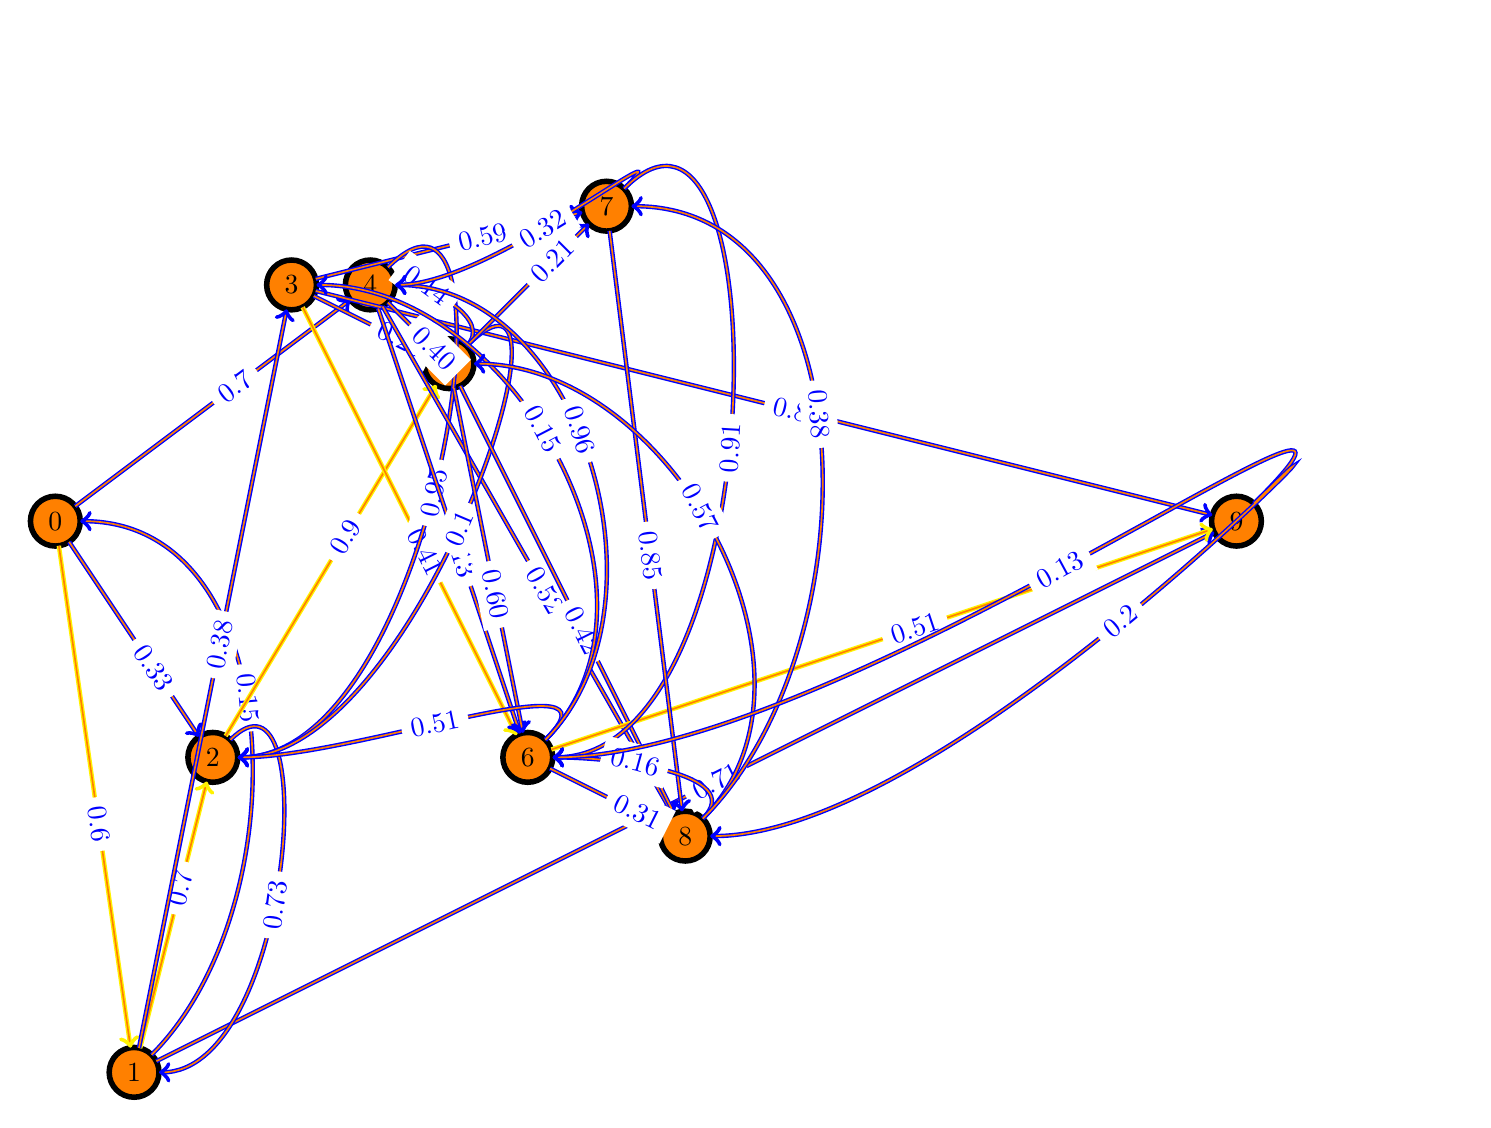
\begin{tikzpicture}
\SetVertexNormal[Shape      = circle,
FillColor  = orange,
LineWidth  = 2pt]
\SetUpEdge[lw         = 0.5pt,
color      = black,
labelcolor = white,
labeltext  = red,
labelstyle = {sloped,text=blue}]
\tikzstyle{TempStyle}=[double = orange]
\Vertex[x=-10, y=8]{0}
\Vertex[x=-9, y=1]{1}
\Vertex[x=-8, y=5]{2}
\Vertex[x=-7, y=11]{3}
\Vertex[x=-6, y=11]{4}
\Vertex[x=-5, y=10]{5}
\Vertex[x=-4, y=5]{6}
\Vertex[x=-3, y=12]{7}
\Vertex[x=-2, y=4]{8}
\Vertex[x=5, y=8]{9}
\tikzset{EdgeStyle/.style={->,TempStyle,relative=false,right=60,color=yellow}}
\Edge[label=$0.6$](0)(1)
\tikzset{EdgeStyle/.style={->,TempStyle,relative=false,right=60,color=blue}}
\Edge[label=$0.33$](0)(2)
\tikzset{EdgeStyle/.style={->,TempStyle,relative=false,right=60,color=blue}}
\Edge[label=$0.7$](0)(4)
\tikzset{EdgeStyle/.style={->,TempStyle,relative=false,left=60,color=blue,in=0,draw}}
\Edge[label=$0.15$](1)(0)
\tikzset{EdgeStyle/.style={->,TempStyle,relative=false,right=60,color=yellow}}
\Edge[label=$0.7$](1)(2)
\tikzset{EdgeStyle/.style={->,TempStyle,relative=false,right=60,color=blue}}
\Edge[label=$0.38$](1)(3)
\tikzset{EdgeStyle/.style={->,TempStyle,relative=false,right=60,color=blue}}
\Edge[label=$0.71$](1)(9)
\tikzset{EdgeStyle/.style={->,TempStyle,relative=false,left=60,color=blue,in=0,draw}}
\Edge[label=$0.73$](2)(1)
\tikzset{EdgeStyle/.style={->,TempStyle,relative=false,right=60,color=yellow}}
\Edge[label=$0.9$](2)(5)
\tikzset{EdgeStyle/.style={->,TempStyle,relative=false,right=60,color=blue}}
\Edge[label=$0.23$](3)(5)
\tikzset{EdgeStyle/.style={->,TempStyle,relative=false,right=60,color=yellow}}
\Edge[label=$0.41$](3)(6)
\tikzset{EdgeStyle/.style={->,TempStyle,relative=false,right=60,color=blue}}
\Edge[label=$0.59$](3)(7)
\tikzset{EdgeStyle/.style={->,TempStyle,relative=false,right=60,color=blue}}
\Edge[label=$0.8$](3)(9)
\tikzset{EdgeStyle/.style={->,TempStyle,relative=false,left=60,color=blue,in=0,draw}}
\Edge[label=$0.95$](4)(2)
\tikzset{EdgeStyle/.style={->,TempStyle,relative=false,right=60,color=blue}}
\Edge[label=$0.40$](4)(5)
\tikzset{EdgeStyle/.style={->,TempStyle,relative=false,right=60,color=blue}}
\Edge[label=$0.13$](4)(6)
\tikzset{EdgeStyle/.style={->,TempStyle,relative=false,right=60,color=blue}}
\Edge[label=$0.52$](4)(8)
\tikzset{EdgeStyle/.style={->,TempStyle,relative=false,left=60,color=blue,in=0,draw}}
\Edge[label=$0.1$](5)(2)
\tikzset{EdgeStyle/.style={->,TempStyle,relative=false,left=60,color=blue,in=0,draw}}
\Edge[label=$0.14$](5)(4)
\tikzset{EdgeStyle/.style={->,TempStyle,relative=false,right=60,color=blue}}
\Edge[label=$0.60$](5)(6)
\tikzset{EdgeStyle/.style={->,TempStyle,relative=false,right=60,color=blue}}
\Edge[label=$0.21$](5)(7)
\tikzset{EdgeStyle/.style={->,TempStyle,relative=false,right=60,color=blue}}
\Edge[label=$0.42$](5)(8)
\tikzset{EdgeStyle/.style={->,TempStyle,relative=false,left=60,color=blue,in=0,draw}}
\Edge[label=$0.51$](6)(2)
\tikzset{EdgeStyle/.style={->,TempStyle,relative=false,left=60,color=blue,in=0,draw}}
\Edge[label=$0.15$](6)(3)
\tikzset{EdgeStyle/.style={->,TempStyle,relative=false,left=60,color=blue,in=0,draw}}
\Edge[label=$0.96$](6)(4)
\tikzset{EdgeStyle/.style={->,TempStyle,relative=false,right=60,color=blue}}
\Edge[label=$0.31$](6)(8)
\tikzset{EdgeStyle/.style={->,TempStyle,relative=false,right=60,color=yellow}}
\Edge[label=$0.51$](6)(9)
\tikzset{EdgeStyle/.style={->,TempStyle,relative=false,left=60,color=blue,in=0,draw}}
\Edge[label=$0.32$](7)(4)
\tikzset{EdgeStyle/.style={->,TempStyle,relative=false,left=60,color=blue,in=0,draw}}
\Edge[label=$0.91$](7)(6)
\tikzset{EdgeStyle/.style={->,TempStyle,relative=false,right=60,color=blue}}
\Edge[label=$0.85$](7)(8)
\tikzset{EdgeStyle/.style={->,TempStyle,relative=false,left=60,color=blue,in=0,draw}}
\Edge[label=$0.57$](8)(5)
\tikzset{EdgeStyle/.style={->,TempStyle,relative=false,left=60,color=blue,in=0,draw}}
\Edge[label=$0.16$](8)(6)
\tikzset{EdgeStyle/.style={->,TempStyle,relative=false,left=60,color=blue,in=0,draw}}
\Edge[label=$0.38$](8)(7)
\tikzset{EdgeStyle/.style={->,TempStyle,relative=false,left=60,color=blue,in=0,draw}}
\Edge[label=$0.13$](9)(6)
\tikzset{EdgeStyle/.style={->,TempStyle,relative=false,left=60,color=blue,in=0,draw}}
\Edge[label=$0.2$](9)(8)
\end{tikzpicture}\\
\begin{center}\begin{tabular}{l c}\\
\textcolor{orange}{\LARGE$\rightarrow$} & Chemin \\
 \textcolor{red}{\LARGE$\rightarrow$} & Créations arcs\\
 \textcolor{green}{\LARGE$\rightarrow$} & Modification flot\\
\end{tabular}
\end{center}
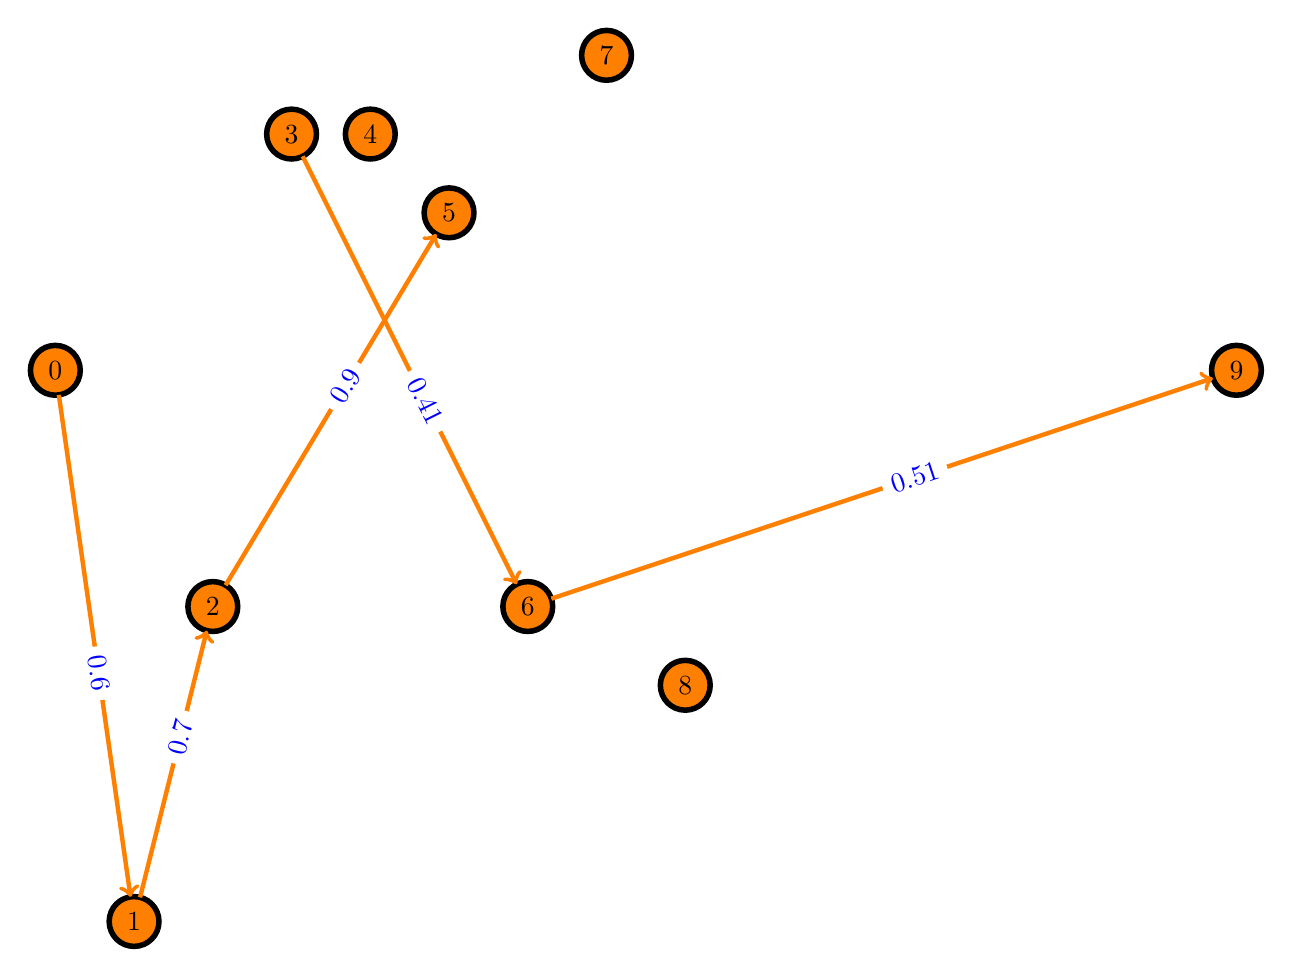
\begin{tikzpicture}
\SetVertexNormal[Shape      = circle,
FillColor  = orange,
LineWidth  = 2pt]
\SetUpEdge[lw         = 0.5pt,
color      = black,
labelcolor = white,
labeltext  = red,
labelstyle = {sloped,text=blue}]
\tikzstyle{TempStyle}=[double = orange]
\Vertex[x=-10, y=8]{0}
\Vertex[x=-9, y=1]{1}
\Vertex[x=-8, y=5]{2}
\Vertex[x=-7, y=11]{3}
\Vertex[x=-6, y=11]{4}
\Vertex[x=-5, y=10]{5}
\Vertex[x=-4, y=5]{6}
\Vertex[x=-3, y=12]{7}
\Vertex[x=-2, y=4]{8}
\Vertex[x=5, y=8]{9}
\tikzset{EdgeStyle/.style={->,TempStyle,relative=false,right=60,color=orange}}
\Edge[label=$0.6$](0)(1)
\tikzset{EdgeStyle/.style={->,TempStyle,relative=false,right=60,color=orange}}
\Edge[label=$0.7$](1)(2)
\tikzset{EdgeStyle/.style={->,TempStyle,relative=false,right=60,color=orange}}
\Edge[label=$0.9$](2)(5)
\tikzset{EdgeStyle/.style={->,TempStyle,relative=false,right=60,color=orange}}
\Edge[label=$0.41$](3)(6)
\tikzset{EdgeStyle/.style={->,TempStyle,relative=false,right=60,color=orange}}
\Edge[label=$0.51$](6)(9)
\end{tikzpicture}\\
\begin{center}\begin{tabular}{l c}\\
\textcolor{orange}{\LARGE$\rightarrow$} & Chemin \\
 \textcolor{red}{\LARGE$\rightarrow$} & Créations arcs\\
 \textcolor{green}{\LARGE$\rightarrow$} & Modification flot\\
\end{tabular}
\end{center}
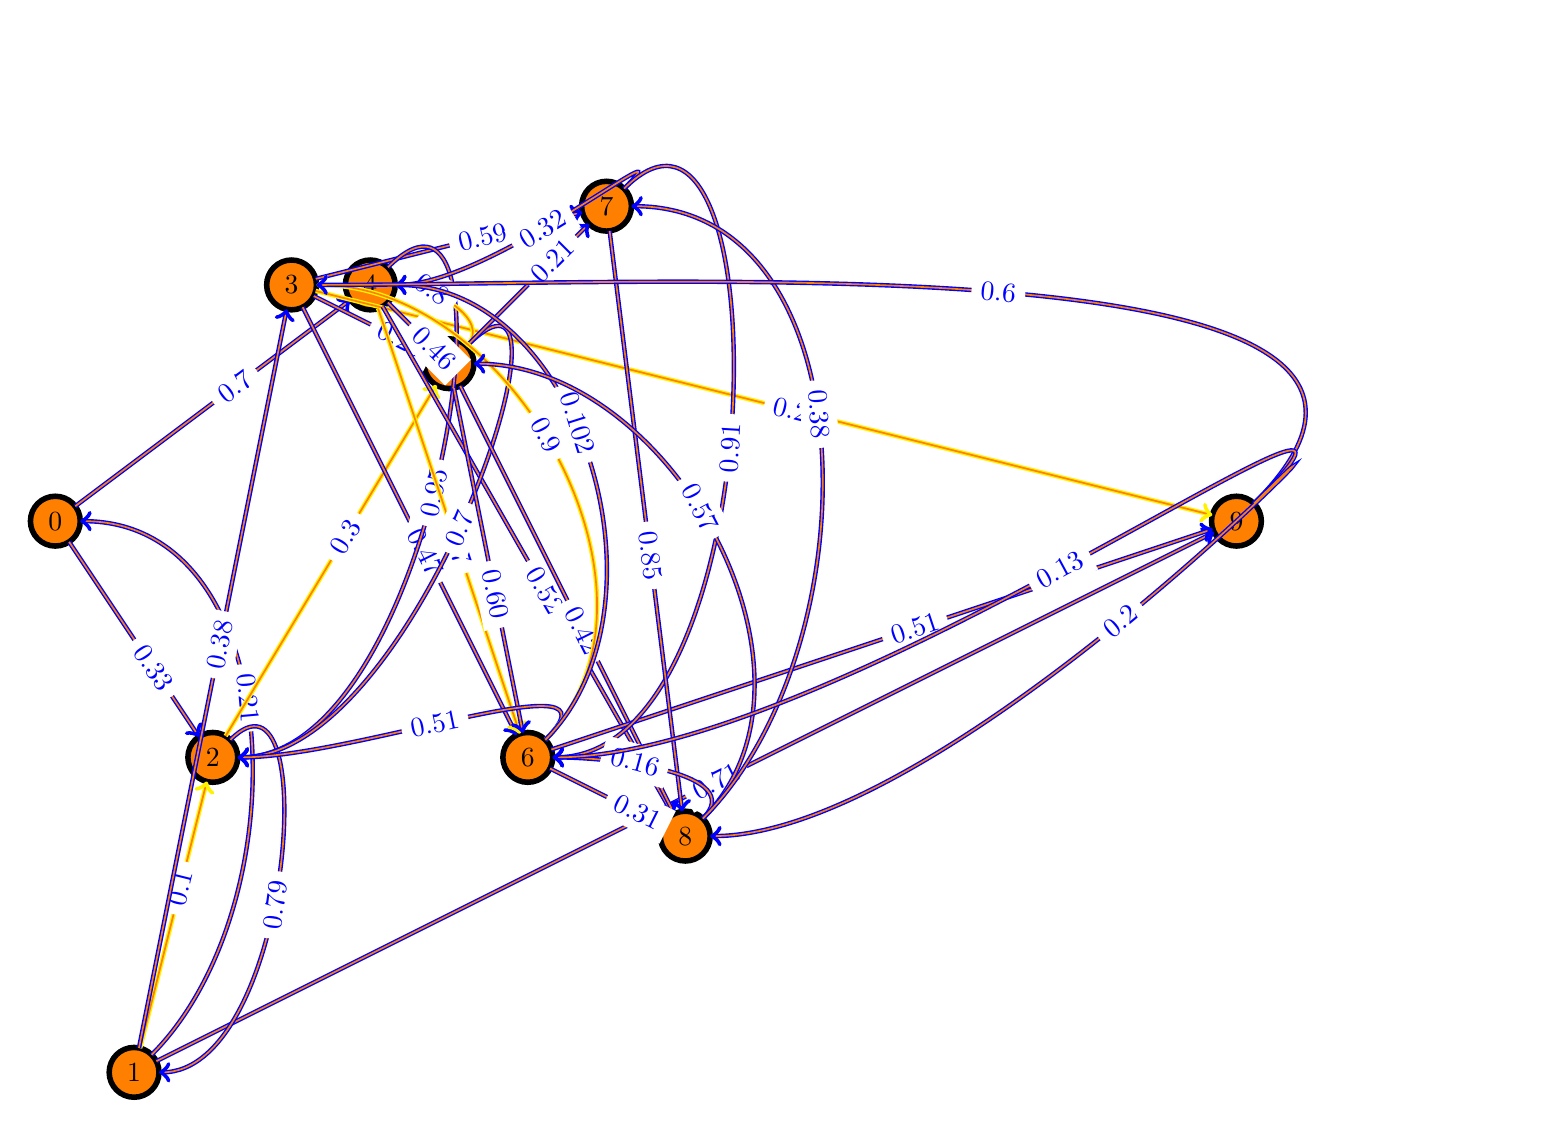
\begin{tikzpicture}
\SetVertexNormal[Shape      = circle,
FillColor  = orange,
LineWidth  = 2pt]
\SetUpEdge[lw         = 0.5pt,
color      = black,
labelcolor = white,
labeltext  = red,
labelstyle = {sloped,text=blue}]
\tikzstyle{TempStyle}=[double = orange]
\Vertex[x=-10, y=8]{0}
\Vertex[x=-9, y=1]{1}
\Vertex[x=-8, y=5]{2}
\Vertex[x=-7, y=11]{3}
\Vertex[x=-6, y=11]{4}
\Vertex[x=-5, y=10]{5}
\Vertex[x=-4, y=5]{6}
\Vertex[x=-3, y=12]{7}
\Vertex[x=-2, y=4]{8}
\Vertex[x=5, y=8]{9}
\tikzset{EdgeStyle/.style={->,TempStyle,relative=false,right=60,color=blue}}
\Edge[label=$0.33$](0)(2)
\tikzset{EdgeStyle/.style={->,TempStyle,relative=false,right=60,color=blue}}
\Edge[label=$0.7$](0)(4)
\tikzset{EdgeStyle/.style={->,TempStyle,relative=false,left=60,color=blue,in=0,draw}}
\Edge[label=$0.21$](1)(0)
\tikzset{EdgeStyle/.style={->,TempStyle,relative=false,right=60,color=yellow}}
\Edge[label=$0.1$](1)(2)
\tikzset{EdgeStyle/.style={->,TempStyle,relative=false,right=60,color=blue}}
\Edge[label=$0.38$](1)(3)
\tikzset{EdgeStyle/.style={->,TempStyle,relative=false,right=60,color=blue}}
\Edge[label=$0.71$](1)(9)
\tikzset{EdgeStyle/.style={->,TempStyle,relative=false,left=60,color=blue,in=0,draw}}
\Edge[label=$0.79$](2)(1)
\tikzset{EdgeStyle/.style={->,TempStyle,relative=false,right=60,color=yellow}}
\Edge[label=$0.3$](2)(5)
\tikzset{EdgeStyle/.style={->,TempStyle,relative=false,right=60,color=blue}}
\Edge[label=$0.23$](3)(5)
\tikzset{EdgeStyle/.style={->,TempStyle,relative=false,right=60,color=blue}}
\Edge[label=$0.47$](3)(6)
\tikzset{EdgeStyle/.style={->,TempStyle,relative=false,right=60,color=blue}}
\Edge[label=$0.59$](3)(7)
\tikzset{EdgeStyle/.style={->,TempStyle,relative=false,right=60,color=yellow}}
\Edge[label=$0.2$](3)(9)
\tikzset{EdgeStyle/.style={->,TempStyle,relative=false,left=60,color=blue,in=0,draw}}
\Edge[label=$0.95$](4)(2)
\tikzset{EdgeStyle/.style={->,TempStyle,relative=false,right=60,color=blue}}
\Edge[label=$0.46$](4)(5)
\tikzset{EdgeStyle/.style={->,TempStyle,relative=false,right=60,color=yellow}}
\Edge[label=$0.7$](4)(6)
\tikzset{EdgeStyle/.style={->,TempStyle,relative=false,right=60,color=blue}}
\Edge[label=$0.52$](4)(8)
\tikzset{EdgeStyle/.style={->,TempStyle,relative=false,left=60,color=blue,in=0,draw}}
\Edge[label=$0.7$](5)(2)
\tikzset{EdgeStyle/.style={->,TempStyle,relative=false,left=60,in=0,color=yellow}}
\Edge[label=$0.8$](5)(4)
\tikzset{EdgeStyle/.style={->,TempStyle,relative=false,right=60,color=blue}}
\Edge[label=$0.60$](5)(6)
\tikzset{EdgeStyle/.style={->,TempStyle,relative=false,right=60,color=blue}}
\Edge[label=$0.21$](5)(7)
\tikzset{EdgeStyle/.style={->,TempStyle,relative=false,right=60,color=blue}}
\Edge[label=$0.42$](5)(8)
\tikzset{EdgeStyle/.style={->,TempStyle,relative=false,left=60,color=blue,in=0,draw}}
\Edge[label=$0.51$](6)(2)
\tikzset{EdgeStyle/.style={->,TempStyle,relative=false,left=60,in=0,color=yellow}}
\Edge[label=$0.9$](6)(3)
\tikzset{EdgeStyle/.style={->,TempStyle,relative=false,left=60,color=blue,in=0,draw}}
\Edge[label=$0.102$](6)(4)
\tikzset{EdgeStyle/.style={->,TempStyle,relative=false,right=60,color=blue}}
\Edge[label=$0.31$](6)(8)
\tikzset{EdgeStyle/.style={->,TempStyle,relative=false,right=60,color=blue}}
\Edge[label=$0.51$](6)(9)
\tikzset{EdgeStyle/.style={->,TempStyle,relative=false,left=60,color=blue,in=0,draw}}
\Edge[label=$0.32$](7)(4)
\tikzset{EdgeStyle/.style={->,TempStyle,relative=false,left=60,color=blue,in=0,draw}}
\Edge[label=$0.91$](7)(6)
\tikzset{EdgeStyle/.style={->,TempStyle,relative=false,right=60,color=blue}}
\Edge[label=$0.85$](7)(8)
\tikzset{EdgeStyle/.style={->,TempStyle,relative=false,left=60,color=blue,in=0,draw}}
\Edge[label=$0.57$](8)(5)
\tikzset{EdgeStyle/.style={->,TempStyle,relative=false,left=60,color=blue,in=0,draw}}
\Edge[label=$0.16$](8)(6)
\tikzset{EdgeStyle/.style={->,TempStyle,relative=false,left=60,color=blue,in=0,draw}}
\Edge[label=$0.38$](8)(7)
\tikzset{EdgeStyle/.style={->,TempStyle,relative=false,left=60,color=blue,in=0,draw}}
\Edge[label=$0.6$](9)(3)
\tikzset{EdgeStyle/.style={->,TempStyle,relative=false,left=60,color=blue,in=0,draw}}
\Edge[label=$0.13$](9)(6)
\tikzset{EdgeStyle/.style={->,TempStyle,relative=false,left=60,color=blue,in=0,draw}}
\Edge[label=$0.2$](9)(8)
\end{tikzpicture}\\
\begin{center}\begin{tabular}{l c}\\
\textcolor{orange}{\LARGE$\rightarrow$} & Chemin \\
 \textcolor{red}{\LARGE$\rightarrow$} & Créations arcs\\
 \textcolor{green}{\LARGE$\rightarrow$} & Modification flot\\
\end{tabular}
\end{center}
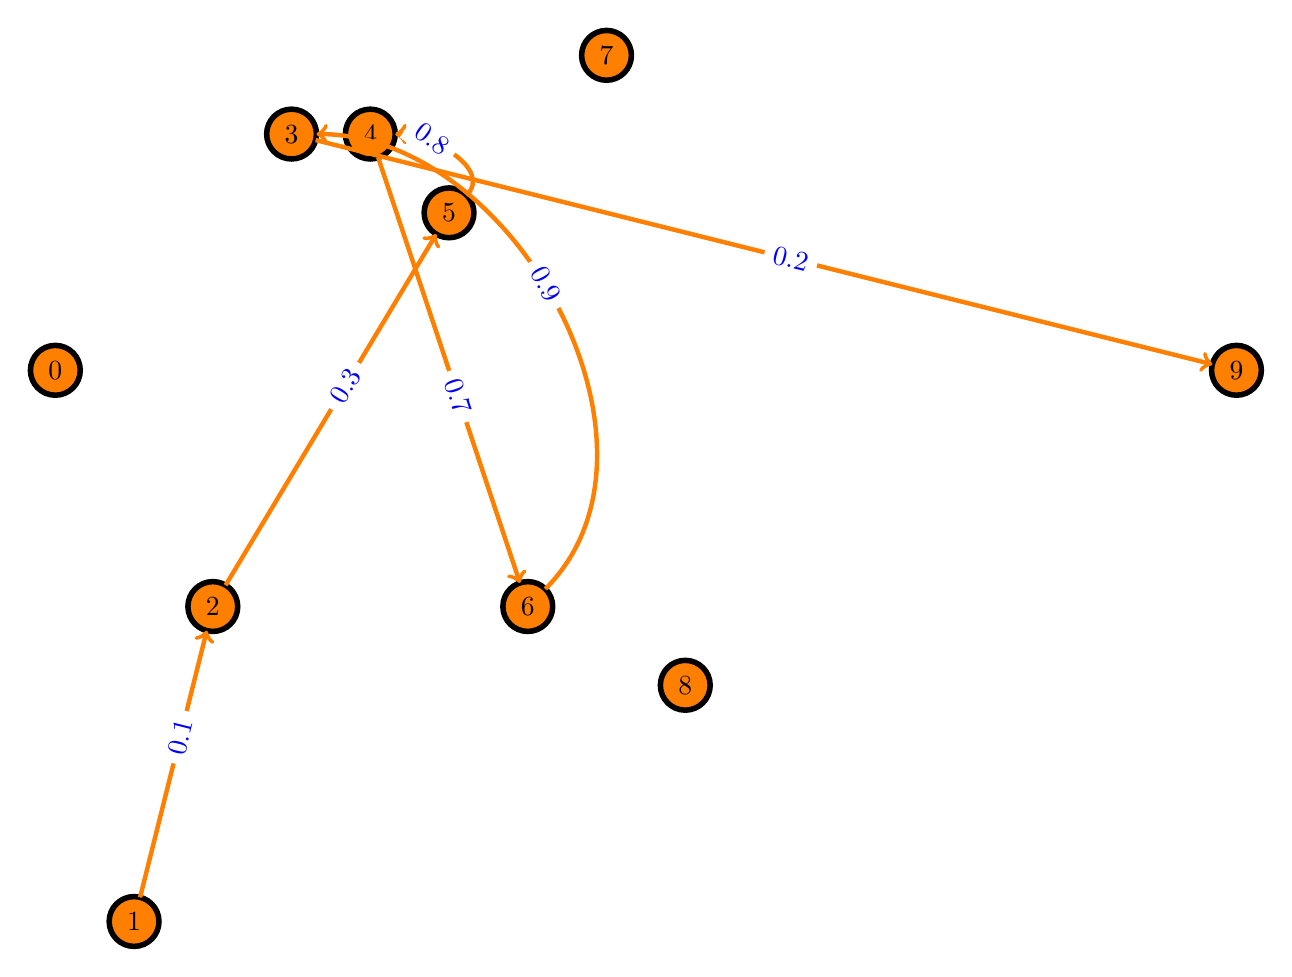
\begin{tikzpicture}
\SetVertexNormal[Shape      = circle,
FillColor  = orange,
LineWidth  = 2pt]
\SetUpEdge[lw         = 0.5pt,
color      = black,
labelcolor = white,
labeltext  = red,
labelstyle = {sloped,text=blue}]
\tikzstyle{TempStyle}=[double = orange]
\Vertex[x=-10, y=8]{0}
\Vertex[x=-9, y=1]{1}
\Vertex[x=-8, y=5]{2}
\Vertex[x=-7, y=11]{3}
\Vertex[x=-6, y=11]{4}
\Vertex[x=-5, y=10]{5}
\Vertex[x=-4, y=5]{6}
\Vertex[x=-3, y=12]{7}
\Vertex[x=-2, y=4]{8}
\Vertex[x=5, y=8]{9}
\tikzset{EdgeStyle/.style={->,TempStyle,relative=false,right=60,color=orange}}
\Edge[label=$0.1$](1)(2)
\tikzset{EdgeStyle/.style={->,TempStyle,relative=false,right=60,color=orange}}
\Edge[label=$0.3$](2)(5)
\tikzset{EdgeStyle/.style={->,TempStyle,relative=false,right=60,color=orange}}
\Edge[label=$0.2$](3)(9)
\tikzset{EdgeStyle/.style={->,TempStyle,relative=false,right=60,color=orange}}
\Edge[label=$0.7$](4)(6)
\tikzset{EdgeStyle/.style={->,TempStyle,relative=false,left=60,color=orange,in=0,draw}}
\Edge[label=$0.8$](5)(4)
\tikzset{EdgeStyle/.style={->,TempStyle,relative=false,left=60,color=orange,in=0,draw}}
\Edge[label=$0.9$](6)(3)
\end{tikzpicture}\\
\begin{center}\begin{tabular}{l c}\\
\textcolor{orange}{\LARGE$\rightarrow$} & Chemin \\
 \textcolor{red}{\LARGE$\rightarrow$} & Créations arcs\\
 \textcolor{green}{\LARGE$\rightarrow$} & Modification flot\\
\end{tabular}
\end{center}
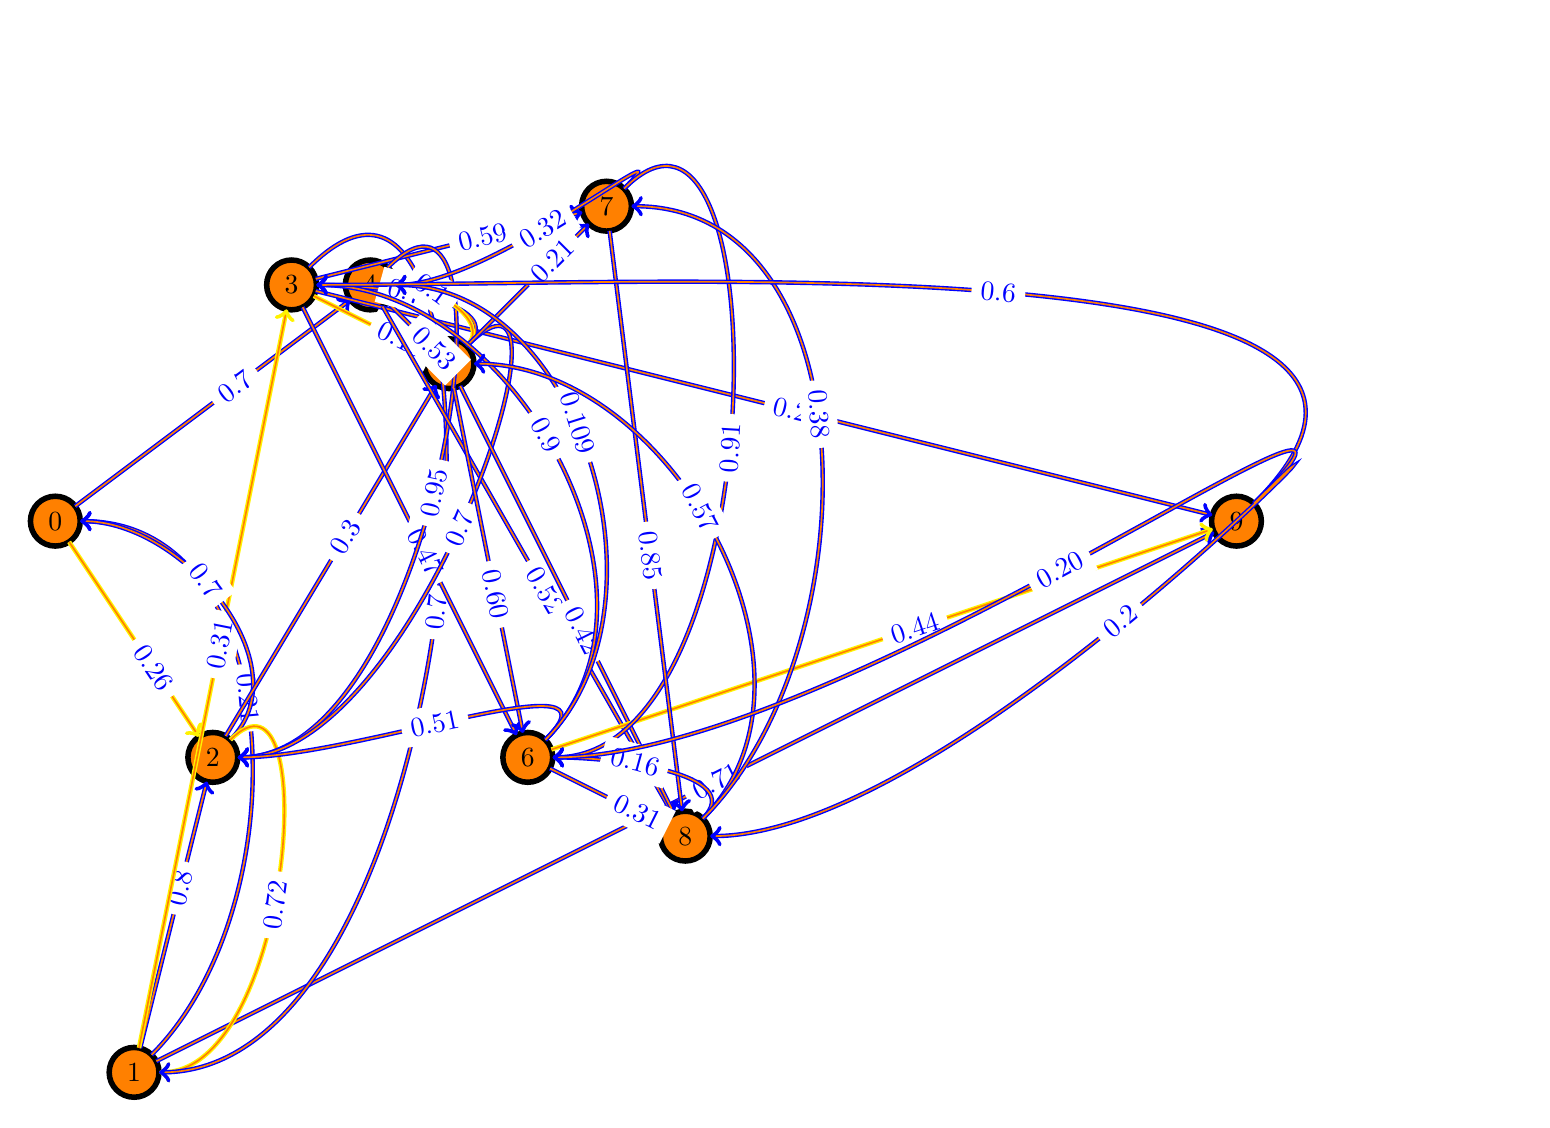
\begin{tikzpicture}
\SetVertexNormal[Shape      = circle,
FillColor  = orange,
LineWidth  = 2pt]
\SetUpEdge[lw         = 0.5pt,
color      = black,
labelcolor = white,
labeltext  = red,
labelstyle = {sloped,text=blue}]
\tikzstyle{TempStyle}=[double = orange]
\Vertex[x=-10, y=8]{0}
\Vertex[x=-9, y=1]{1}
\Vertex[x=-8, y=5]{2}
\Vertex[x=-7, y=11]{3}
\Vertex[x=-6, y=11]{4}
\Vertex[x=-5, y=10]{5}
\Vertex[x=-4, y=5]{6}
\Vertex[x=-3, y=12]{7}
\Vertex[x=-2, y=4]{8}
\Vertex[x=5, y=8]{9}
\tikzset{EdgeStyle/.style={->,TempStyle,relative=false,right=60,color=yellow}}
\Edge[label=$0.26$](0)(2)
\tikzset{EdgeStyle/.style={->,TempStyle,relative=false,right=60,color=blue}}
\Edge[label=$0.7$](0)(4)
\tikzset{EdgeStyle/.style={->,TempStyle,relative=false,left=60,color=blue,in=0,draw}}
\Edge[label=$0.21$](1)(0)
\tikzset{EdgeStyle/.style={->,TempStyle,relative=false,right=60,color=blue}}
\Edge[label=$0.8$](1)(2)
\tikzset{EdgeStyle/.style={->,TempStyle,relative=false,right=60,color=yellow}}
\Edge[label=$0.31$](1)(3)
\tikzset{EdgeStyle/.style={->,TempStyle,relative=false,right=60,color=blue}}
\Edge[label=$0.71$](1)(9)
\tikzset{EdgeStyle/.style={->,TempStyle,relative=false,left=60,color=blue,in=0,draw}}
\Edge[label=$0.7$](2)(0)
\tikzset{EdgeStyle/.style={->,TempStyle,relative=false,left=60,in=0,color=yellow}}
\Edge[label=$0.72$](2)(1)
\tikzset{EdgeStyle/.style={->,TempStyle,relative=false,right=60,color=blue}}
\Edge[label=$0.3$](2)(5)
\tikzset{EdgeStyle/.style={->,TempStyle,relative=false,left=60,color=blue,in=0,draw}}
\Edge[label=$0.7$](3)(1)
\tikzset{EdgeStyle/.style={->,TempStyle,relative=false,right=60,color=yellow}}
\Edge[label=$0.16$](3)(5)
\tikzset{EdgeStyle/.style={->,TempStyle,relative=false,right=60,color=blue}}
\Edge[label=$0.47$](3)(6)
\tikzset{EdgeStyle/.style={->,TempStyle,relative=false,right=60,color=blue}}
\Edge[label=$0.59$](3)(7)
\tikzset{EdgeStyle/.style={->,TempStyle,relative=false,right=60,color=blue}}
\Edge[label=$0.2$](3)(9)
\tikzset{EdgeStyle/.style={->,TempStyle,relative=false,left=60,color=blue,in=0,draw}}
\Edge[label=$0.95$](4)(2)
\tikzset{EdgeStyle/.style={->,TempStyle,relative=false,right=60,color=blue}}
\Edge[label=$0.53$](4)(5)
\tikzset{EdgeStyle/.style={->,TempStyle,relative=false,right=60,color=blue}}
\Edge[label=$0.52$](4)(8)
\tikzset{EdgeStyle/.style={->,TempStyle,relative=false,left=60,color=blue,in=0,draw}}
\Edge[label=$0.7$](5)(2)
\tikzset{EdgeStyle/.style={->,TempStyle,relative=false,left=60,color=blue,in=0,draw}}
\Edge[label=$0.7$](5)(3)
\tikzset{EdgeStyle/.style={->,TempStyle,relative=false,left=60,in=0,color=yellow}}
\Edge[label=$0.1$](5)(4)
\tikzset{EdgeStyle/.style={->,TempStyle,relative=false,right=60,color=blue}}
\Edge[label=$0.60$](5)(6)
\tikzset{EdgeStyle/.style={->,TempStyle,relative=false,right=60,color=blue}}
\Edge[label=$0.21$](5)(7)
\tikzset{EdgeStyle/.style={->,TempStyle,relative=false,right=60,color=blue}}
\Edge[label=$0.42$](5)(8)
\tikzset{EdgeStyle/.style={->,TempStyle,relative=false,left=60,color=blue,in=0,draw}}
\Edge[label=$0.51$](6)(2)
\tikzset{EdgeStyle/.style={->,TempStyle,relative=false,left=60,color=blue,in=0,draw}}
\Edge[label=$0.9$](6)(3)
\tikzset{EdgeStyle/.style={->,TempStyle,relative=false,left=60,color=blue,in=0,draw}}
\Edge[label=$0.109$](6)(4)
\tikzset{EdgeStyle/.style={->,TempStyle,relative=false,right=60,color=blue}}
\Edge[label=$0.31$](6)(8)
\tikzset{EdgeStyle/.style={->,TempStyle,relative=false,right=60,color=yellow}}
\Edge[label=$0.44$](6)(9)
\tikzset{EdgeStyle/.style={->,TempStyle,relative=false,left=60,color=blue,in=0,draw}}
\Edge[label=$0.32$](7)(4)
\tikzset{EdgeStyle/.style={->,TempStyle,relative=false,left=60,color=blue,in=0,draw}}
\Edge[label=$0.91$](7)(6)
\tikzset{EdgeStyle/.style={->,TempStyle,relative=false,right=60,color=blue}}
\Edge[label=$0.85$](7)(8)
\tikzset{EdgeStyle/.style={->,TempStyle,relative=false,left=60,color=blue,in=0,draw}}
\Edge[label=$0.57$](8)(5)
\tikzset{EdgeStyle/.style={->,TempStyle,relative=false,left=60,color=blue,in=0,draw}}
\Edge[label=$0.16$](8)(6)
\tikzset{EdgeStyle/.style={->,TempStyle,relative=false,left=60,color=blue,in=0,draw}}
\Edge[label=$0.38$](8)(7)
\tikzset{EdgeStyle/.style={->,TempStyle,relative=false,left=60,color=blue,in=0,draw}}
\Edge[label=$0.6$](9)(3)
\tikzset{EdgeStyle/.style={->,TempStyle,relative=false,left=60,color=blue,in=0,draw}}
\Edge[label=$0.20$](9)(6)
\tikzset{EdgeStyle/.style={->,TempStyle,relative=false,left=60,color=blue,in=0,draw}}
\Edge[label=$0.2$](9)(8)
\end{tikzpicture}\\
\begin{center}\begin{tabular}{l c}\\
\textcolor{orange}{\LARGE$\rightarrow$} & Chemin \\
 \textcolor{red}{\LARGE$\rightarrow$} & Créations arcs\\
 \textcolor{green}{\LARGE$\rightarrow$} & Modification flot\\
\end{tabular}
\end{center}
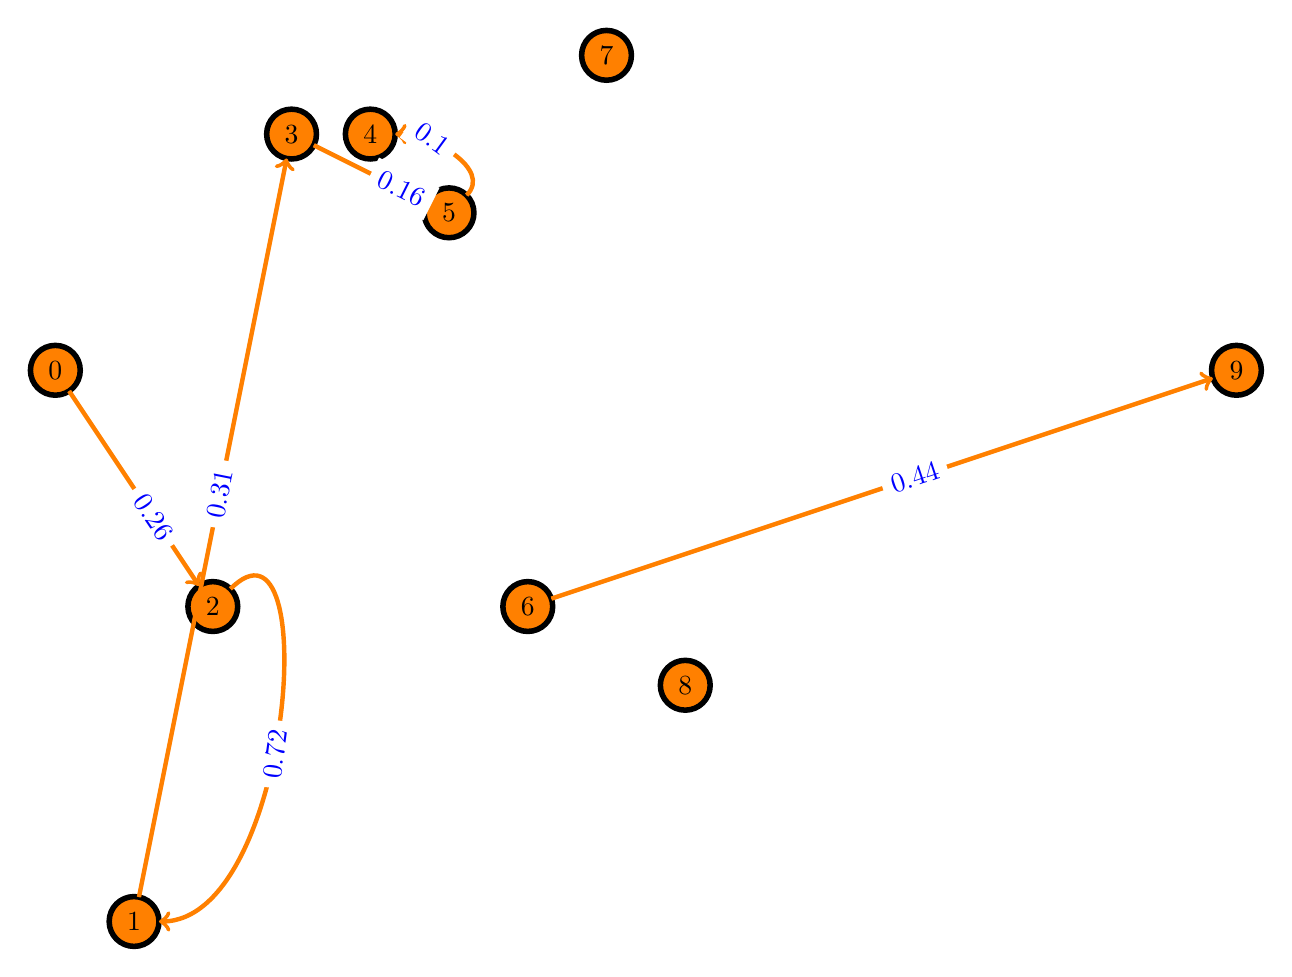
\begin{tikzpicture}
\SetVertexNormal[Shape      = circle,
FillColor  = orange,
LineWidth  = 2pt]
\SetUpEdge[lw         = 0.5pt,
color      = black,
labelcolor = white,
labeltext  = red,
labelstyle = {sloped,text=blue}]
\tikzstyle{TempStyle}=[double = orange]
\Vertex[x=-10, y=8]{0}
\Vertex[x=-9, y=1]{1}
\Vertex[x=-8, y=5]{2}
\Vertex[x=-7, y=11]{3}
\Vertex[x=-6, y=11]{4}
\Vertex[x=-5, y=10]{5}
\Vertex[x=-4, y=5]{6}
\Vertex[x=-3, y=12]{7}
\Vertex[x=-2, y=4]{8}
\Vertex[x=5, y=8]{9}
\tikzset{EdgeStyle/.style={->,TempStyle,relative=false,right=60,color=orange}}
\Edge[label=$0.26$](0)(2)
\tikzset{EdgeStyle/.style={->,TempStyle,relative=false,right=60,color=orange}}
\Edge[label=$0.31$](1)(3)
\tikzset{EdgeStyle/.style={->,TempStyle,relative=false,left=60,color=orange,in=0,draw}}
\Edge[label=$0.72$](2)(1)
\tikzset{EdgeStyle/.style={->,TempStyle,relative=false,right=60,color=orange}}
\Edge[label=$0.16$](3)(5)
\tikzset{EdgeStyle/.style={->,TempStyle,relative=false,left=60,color=orange,in=0,draw}}
\Edge[label=$0.1$](5)(4)
\tikzset{EdgeStyle/.style={->,TempStyle,relative=false,right=60,color=orange}}
\Edge[label=$0.44$](6)(9)
\end{tikzpicture}\\
\begin{center}\begin{tabular}{l c}\\
\textcolor{orange}{\LARGE$\rightarrow$} & Chemin \\
 \textcolor{red}{\LARGE$\rightarrow$} & Créations arcs\\
 \textcolor{green}{\LARGE$\rightarrow$} & Modification flot\\
\end{tabular}
\end{center}
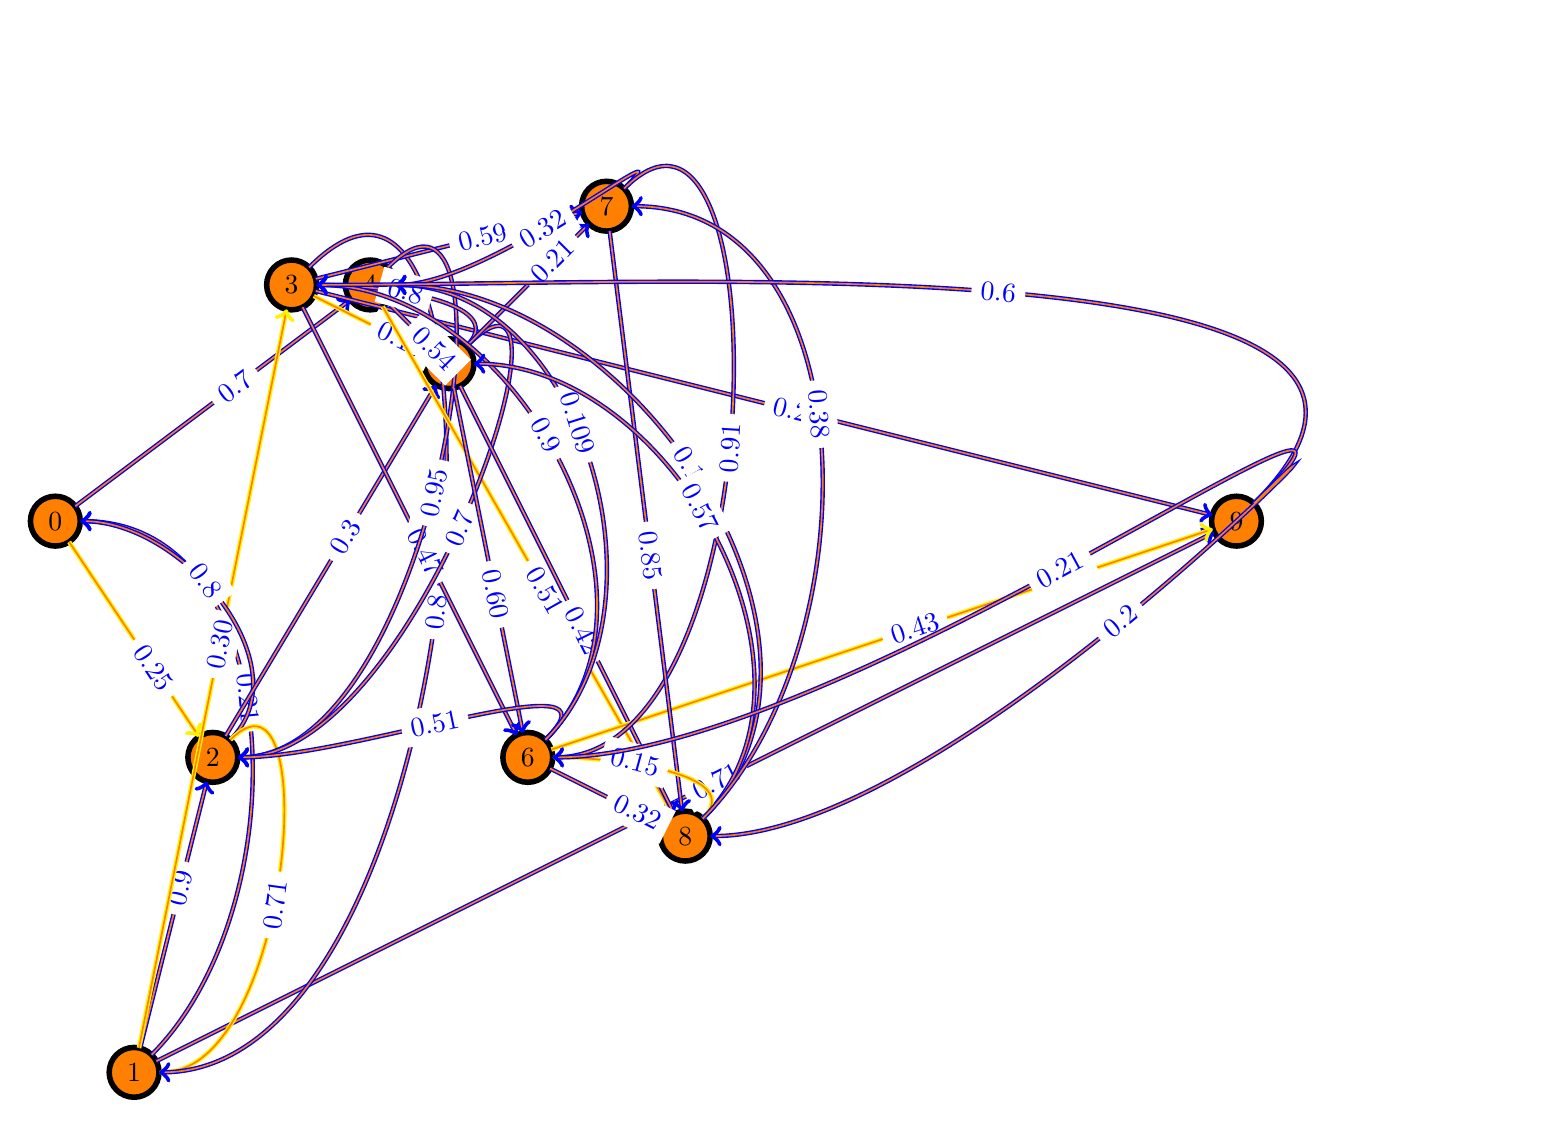
\begin{tikzpicture}
\SetVertexNormal[Shape      = circle,
FillColor  = orange,
LineWidth  = 2pt]
\SetUpEdge[lw         = 0.5pt,
color      = black,
labelcolor = white,
labeltext  = red,
labelstyle = {sloped,text=blue}]
\tikzstyle{TempStyle}=[double = orange]
\Vertex[x=-10, y=8]{0}
\Vertex[x=-9, y=1]{1}
\Vertex[x=-8, y=5]{2}
\Vertex[x=-7, y=11]{3}
\Vertex[x=-6, y=11]{4}
\Vertex[x=-5, y=10]{5}
\Vertex[x=-4, y=5]{6}
\Vertex[x=-3, y=12]{7}
\Vertex[x=-2, y=4]{8}
\Vertex[x=5, y=8]{9}
\tikzset{EdgeStyle/.style={->,TempStyle,relative=false,right=60,color=yellow}}
\Edge[label=$0.25$](0)(2)
\tikzset{EdgeStyle/.style={->,TempStyle,relative=false,right=60,color=blue}}
\Edge[label=$0.7$](0)(4)
\tikzset{EdgeStyle/.style={->,TempStyle,relative=false,left=60,color=blue,in=0,draw}}
\Edge[label=$0.21$](1)(0)
\tikzset{EdgeStyle/.style={->,TempStyle,relative=false,right=60,color=blue}}
\Edge[label=$0.9$](1)(2)
\tikzset{EdgeStyle/.style={->,TempStyle,relative=false,right=60,color=yellow}}
\Edge[label=$0.30$](1)(3)
\tikzset{EdgeStyle/.style={->,TempStyle,relative=false,right=60,color=blue}}
\Edge[label=$0.71$](1)(9)
\tikzset{EdgeStyle/.style={->,TempStyle,relative=false,left=60,color=blue,in=0,draw}}
\Edge[label=$0.8$](2)(0)
\tikzset{EdgeStyle/.style={->,TempStyle,relative=false,left=60,in=0,color=yellow}}
\Edge[label=$0.71$](2)(1)
\tikzset{EdgeStyle/.style={->,TempStyle,relative=false,right=60,color=blue}}
\Edge[label=$0.3$](2)(5)
\tikzset{EdgeStyle/.style={->,TempStyle,relative=false,left=60,color=blue,in=0,draw}}
\Edge[label=$0.8$](3)(1)
\tikzset{EdgeStyle/.style={->,TempStyle,relative=false,right=60,color=yellow}}
\Edge[label=$0.15$](3)(5)
\tikzset{EdgeStyle/.style={->,TempStyle,relative=false,right=60,color=blue}}
\Edge[label=$0.47$](3)(6)
\tikzset{EdgeStyle/.style={->,TempStyle,relative=false,right=60,color=blue}}
\Edge[label=$0.59$](3)(7)
\tikzset{EdgeStyle/.style={->,TempStyle,relative=false,right=60,color=blue}}
\Edge[label=$0.2$](3)(9)
\tikzset{EdgeStyle/.style={->,TempStyle,relative=false,left=60,color=blue,in=0,draw}}
\Edge[label=$0.95$](4)(2)
\tikzset{EdgeStyle/.style={->,TempStyle,relative=false,right=60,color=blue}}
\Edge[label=$0.54$](4)(5)
\tikzset{EdgeStyle/.style={->,TempStyle,relative=false,right=60,color=yellow}}
\Edge[label=$0.51$](4)(8)
\tikzset{EdgeStyle/.style={->,TempStyle,relative=false,left=60,color=blue,in=0,draw}}
\Edge[label=$0.7$](5)(2)
\tikzset{EdgeStyle/.style={->,TempStyle,relative=false,left=60,color=blue,in=0,draw}}
\Edge[label=$0.8$](5)(3)
\tikzset{EdgeStyle/.style={->,TempStyle,relative=false,right=60,color=blue}}
\Edge[label=$0.60$](5)(6)
\tikzset{EdgeStyle/.style={->,TempStyle,relative=false,right=60,color=blue}}
\Edge[label=$0.21$](5)(7)
\tikzset{EdgeStyle/.style={->,TempStyle,relative=false,right=60,color=blue}}
\Edge[label=$0.42$](5)(8)
\tikzset{EdgeStyle/.style={->,TempStyle,relative=false,left=60,color=blue,in=0,draw}}
\Edge[label=$0.51$](6)(2)
\tikzset{EdgeStyle/.style={->,TempStyle,relative=false,left=60,color=blue,in=0,draw}}
\Edge[label=$0.9$](6)(3)
\tikzset{EdgeStyle/.style={->,TempStyle,relative=false,left=60,color=blue,in=0,draw}}
\Edge[label=$0.109$](6)(4)
\tikzset{EdgeStyle/.style={->,TempStyle,relative=false,right=60,color=blue}}
\Edge[label=$0.32$](6)(8)
\tikzset{EdgeStyle/.style={->,TempStyle,relative=false,right=60,color=yellow}}
\Edge[label=$0.43$](6)(9)
\tikzset{EdgeStyle/.style={->,TempStyle,relative=false,left=60,color=blue,in=0,draw}}
\Edge[label=$0.32$](7)(4)
\tikzset{EdgeStyle/.style={->,TempStyle,relative=false,left=60,color=blue,in=0,draw}}
\Edge[label=$0.91$](7)(6)
\tikzset{EdgeStyle/.style={->,TempStyle,relative=false,right=60,color=blue}}
\Edge[label=$0.85$](7)(8)
\tikzset{EdgeStyle/.style={->,TempStyle,relative=false,left=60,color=blue,in=0,draw}}
\Edge[label=$0.1$](8)(4)
\tikzset{EdgeStyle/.style={->,TempStyle,relative=false,left=60,color=blue,in=0,draw}}
\Edge[label=$0.57$](8)(5)
\tikzset{EdgeStyle/.style={->,TempStyle,relative=false,left=60,in=0,color=yellow}}
\Edge[label=$0.15$](8)(6)
\tikzset{EdgeStyle/.style={->,TempStyle,relative=false,left=60,color=blue,in=0,draw}}
\Edge[label=$0.38$](8)(7)
\tikzset{EdgeStyle/.style={->,TempStyle,relative=false,left=60,color=blue,in=0,draw}}
\Edge[label=$0.6$](9)(3)
\tikzset{EdgeStyle/.style={->,TempStyle,relative=false,left=60,color=blue,in=0,draw}}
\Edge[label=$0.21$](9)(6)
\tikzset{EdgeStyle/.style={->,TempStyle,relative=false,left=60,color=blue,in=0,draw}}
\Edge[label=$0.2$](9)(8)
\end{tikzpicture}\\
\begin{center}\begin{tabular}{l c}\\
\textcolor{orange}{\LARGE$\rightarrow$} & Chemin \\
 \textcolor{red}{\LARGE$\rightarrow$} & Créations arcs\\
 \textcolor{green}{\LARGE$\rightarrow$} & Modification flot\\
\end{tabular}
\end{center}
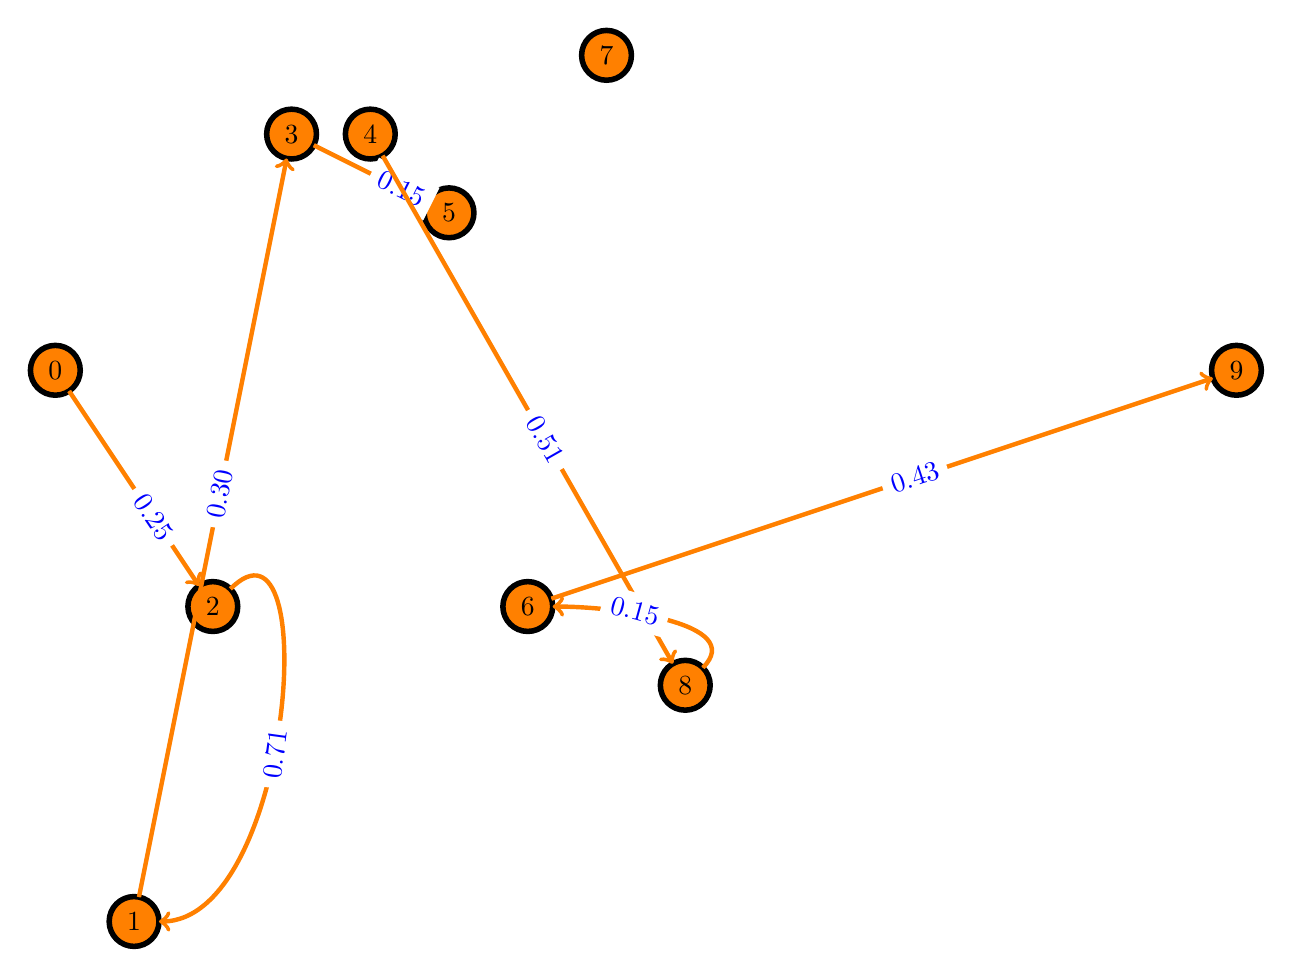
\begin{tikzpicture}
\SetVertexNormal[Shape      = circle,
FillColor  = orange,
LineWidth  = 2pt]
\SetUpEdge[lw         = 0.5pt,
color      = black,
labelcolor = white,
labeltext  = red,
labelstyle = {sloped,text=blue}]
\tikzstyle{TempStyle}=[double = orange]
\Vertex[x=-10, y=8]{0}
\Vertex[x=-9, y=1]{1}
\Vertex[x=-8, y=5]{2}
\Vertex[x=-7, y=11]{3}
\Vertex[x=-6, y=11]{4}
\Vertex[x=-5, y=10]{5}
\Vertex[x=-4, y=5]{6}
\Vertex[x=-3, y=12]{7}
\Vertex[x=-2, y=4]{8}
\Vertex[x=5, y=8]{9}
\tikzset{EdgeStyle/.style={->,TempStyle,relative=false,right=60,color=orange}}
\Edge[label=$0.25$](0)(2)
\tikzset{EdgeStyle/.style={->,TempStyle,relative=false,right=60,color=orange}}
\Edge[label=$0.30$](1)(3)
\tikzset{EdgeStyle/.style={->,TempStyle,relative=false,left=60,color=orange,in=0,draw}}
\Edge[label=$0.71$](2)(1)
\tikzset{EdgeStyle/.style={->,TempStyle,relative=false,right=60,color=orange}}
\Edge[label=$0.15$](3)(5)
\tikzset{EdgeStyle/.style={->,TempStyle,relative=false,right=60,color=orange}}
\Edge[label=$0.51$](4)(8)
\tikzset{EdgeStyle/.style={->,TempStyle,relative=false,right=60,color=orange}}
\Edge[label=$0.43$](6)(9)
\tikzset{EdgeStyle/.style={->,TempStyle,relative=false,left=60,color=orange,in=0,draw}}
\Edge[label=$0.15$](8)(6)
\end{tikzpicture}\\
\begin{center}\begin{tabular}{l c}\\
\textcolor{orange}{\LARGE$\rightarrow$} & Chemin \\
 \textcolor{red}{\LARGE$\rightarrow$} & Créations arcs\\
 \textcolor{green}{\LARGE$\rightarrow$} & Modification flot\\
\end{tabular}
\end{center}
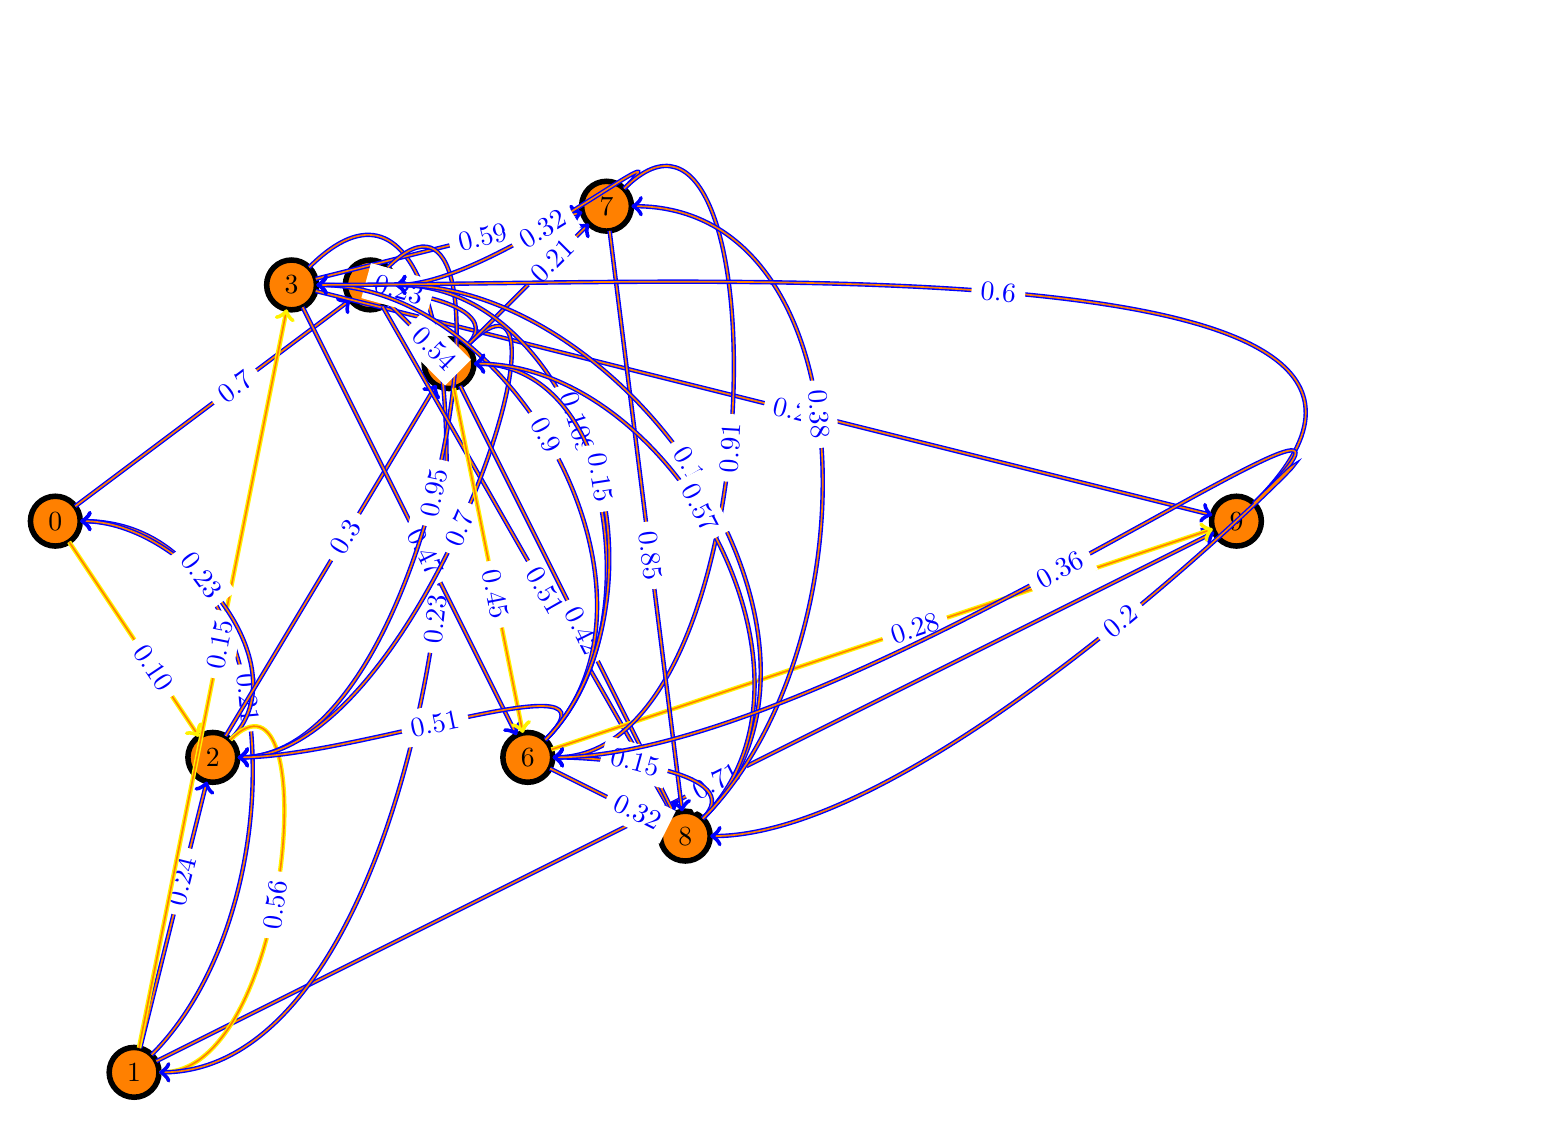
\begin{tikzpicture}
\SetVertexNormal[Shape      = circle,
FillColor  = orange,
LineWidth  = 2pt]
\SetUpEdge[lw         = 0.5pt,
color      = black,
labelcolor = white,
labeltext  = red,
labelstyle = {sloped,text=blue}]
\tikzstyle{TempStyle}=[double = orange]
\Vertex[x=-10, y=8]{0}
\Vertex[x=-9, y=1]{1}
\Vertex[x=-8, y=5]{2}
\Vertex[x=-7, y=11]{3}
\Vertex[x=-6, y=11]{4}
\Vertex[x=-5, y=10]{5}
\Vertex[x=-4, y=5]{6}
\Vertex[x=-3, y=12]{7}
\Vertex[x=-2, y=4]{8}
\Vertex[x=5, y=8]{9}
\tikzset{EdgeStyle/.style={->,TempStyle,relative=false,right=60,color=yellow}}
\Edge[label=$0.10$](0)(2)
\tikzset{EdgeStyle/.style={->,TempStyle,relative=false,right=60,color=blue}}
\Edge[label=$0.7$](0)(4)
\tikzset{EdgeStyle/.style={->,TempStyle,relative=false,left=60,color=blue,in=0,draw}}
\Edge[label=$0.21$](1)(0)
\tikzset{EdgeStyle/.style={->,TempStyle,relative=false,right=60,color=blue}}
\Edge[label=$0.24$](1)(2)
\tikzset{EdgeStyle/.style={->,TempStyle,relative=false,right=60,color=yellow}}
\Edge[label=$0.15$](1)(3)
\tikzset{EdgeStyle/.style={->,TempStyle,relative=false,right=60,color=blue}}
\Edge[label=$0.71$](1)(9)
\tikzset{EdgeStyle/.style={->,TempStyle,relative=false,left=60,color=blue,in=0,draw}}
\Edge[label=$0.23$](2)(0)
\tikzset{EdgeStyle/.style={->,TempStyle,relative=false,left=60,in=0,color=yellow}}
\Edge[label=$0.56$](2)(1)
\tikzset{EdgeStyle/.style={->,TempStyle,relative=false,right=60,color=blue}}
\Edge[label=$0.3$](2)(5)
\tikzset{EdgeStyle/.style={->,TempStyle,relative=false,left=60,color=blue,in=0,draw}}
\Edge[label=$0.23$](3)(1)
\tikzset{EdgeStyle/.style={->,TempStyle,relative=false,right=60,color=blue}}
\Edge[label=$0.47$](3)(6)
\tikzset{EdgeStyle/.style={->,TempStyle,relative=false,right=60,color=blue}}
\Edge[label=$0.59$](3)(7)
\tikzset{EdgeStyle/.style={->,TempStyle,relative=false,right=60,color=blue}}
\Edge[label=$0.2$](3)(9)
\tikzset{EdgeStyle/.style={->,TempStyle,relative=false,left=60,color=blue,in=0,draw}}
\Edge[label=$0.95$](4)(2)
\tikzset{EdgeStyle/.style={->,TempStyle,relative=false,right=60,color=blue}}
\Edge[label=$0.54$](4)(5)
\tikzset{EdgeStyle/.style={->,TempStyle,relative=false,right=60,color=blue}}
\Edge[label=$0.51$](4)(8)
\tikzset{EdgeStyle/.style={->,TempStyle,relative=false,left=60,color=blue,in=0,draw}}
\Edge[label=$0.7$](5)(2)
\tikzset{EdgeStyle/.style={->,TempStyle,relative=false,left=60,color=blue,in=0,draw}}
\Edge[label=$0.23$](5)(3)
\tikzset{EdgeStyle/.style={->,TempStyle,relative=false,right=60,color=yellow}}
\Edge[label=$0.45$](5)(6)
\tikzset{EdgeStyle/.style={->,TempStyle,relative=false,right=60,color=blue}}
\Edge[label=$0.21$](5)(7)
\tikzset{EdgeStyle/.style={->,TempStyle,relative=false,right=60,color=blue}}
\Edge[label=$0.42$](5)(8)
\tikzset{EdgeStyle/.style={->,TempStyle,relative=false,left=60,color=blue,in=0,draw}}
\Edge[label=$0.51$](6)(2)
\tikzset{EdgeStyle/.style={->,TempStyle,relative=false,left=60,color=blue,in=0,draw}}
\Edge[label=$0.9$](6)(3)
\tikzset{EdgeStyle/.style={->,TempStyle,relative=false,left=60,color=blue,in=0,draw}}
\Edge[label=$0.109$](6)(4)
\tikzset{EdgeStyle/.style={->,TempStyle,relative=false,left=60,color=blue,in=0,draw}}
\Edge[label=$0.15$](6)(5)
\tikzset{EdgeStyle/.style={->,TempStyle,relative=false,right=60,color=blue}}
\Edge[label=$0.32$](6)(8)
\tikzset{EdgeStyle/.style={->,TempStyle,relative=false,right=60,color=yellow}}
\Edge[label=$0.28$](6)(9)
\tikzset{EdgeStyle/.style={->,TempStyle,relative=false,left=60,color=blue,in=0,draw}}
\Edge[label=$0.32$](7)(4)
\tikzset{EdgeStyle/.style={->,TempStyle,relative=false,left=60,color=blue,in=0,draw}}
\Edge[label=$0.91$](7)(6)
\tikzset{EdgeStyle/.style={->,TempStyle,relative=false,right=60,color=blue}}
\Edge[label=$0.85$](7)(8)
\tikzset{EdgeStyle/.style={->,TempStyle,relative=false,left=60,color=blue,in=0,draw}}
\Edge[label=$0.1$](8)(4)
\tikzset{EdgeStyle/.style={->,TempStyle,relative=false,left=60,color=blue,in=0,draw}}
\Edge[label=$0.57$](8)(5)
\tikzset{EdgeStyle/.style={->,TempStyle,relative=false,left=60,color=blue,in=0,draw}}
\Edge[label=$0.15$](8)(6)
\tikzset{EdgeStyle/.style={->,TempStyle,relative=false,left=60,color=blue,in=0,draw}}
\Edge[label=$0.38$](8)(7)
\tikzset{EdgeStyle/.style={->,TempStyle,relative=false,left=60,color=blue,in=0,draw}}
\Edge[label=$0.6$](9)(3)
\tikzset{EdgeStyle/.style={->,TempStyle,relative=false,left=60,color=blue,in=0,draw}}
\Edge[label=$0.36$](9)(6)
\tikzset{EdgeStyle/.style={->,TempStyle,relative=false,left=60,color=blue,in=0,draw}}
\Edge[label=$0.2$](9)(8)
\end{tikzpicture}\\
\begin{center}\begin{tabular}{l c}\\
\textcolor{orange}{\LARGE$\rightarrow$} & Chemin \\
 \textcolor{red}{\LARGE$\rightarrow$} & Créations arcs\\
 \textcolor{green}{\LARGE$\rightarrow$} & Modification flot\\
\end{tabular}
\end{center}
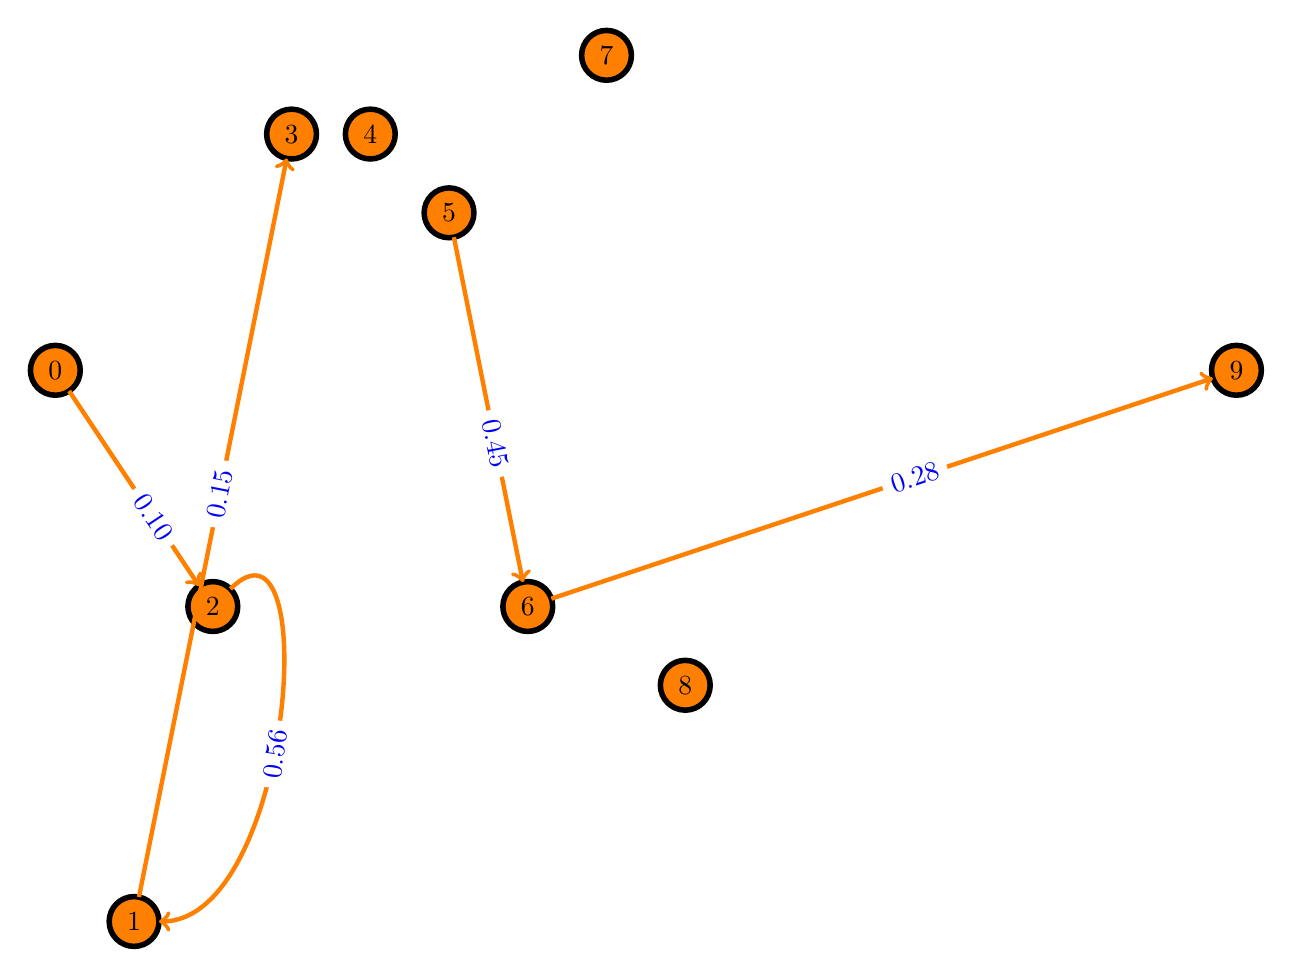
\begin{tikzpicture}
\SetVertexNormal[Shape      = circle,
FillColor  = orange,
LineWidth  = 2pt]
\SetUpEdge[lw         = 0.5pt,
color      = black,
labelcolor = white,
labeltext  = red,
labelstyle = {sloped,text=blue}]
\tikzstyle{TempStyle}=[double = orange]
\Vertex[x=-10, y=8]{0}
\Vertex[x=-9, y=1]{1}
\Vertex[x=-8, y=5]{2}
\Vertex[x=-7, y=11]{3}
\Vertex[x=-6, y=11]{4}
\Vertex[x=-5, y=10]{5}
\Vertex[x=-4, y=5]{6}
\Vertex[x=-3, y=12]{7}
\Vertex[x=-2, y=4]{8}
\Vertex[x=5, y=8]{9}
\tikzset{EdgeStyle/.style={->,TempStyle,relative=false,right=60,color=orange}}
\Edge[label=$0.10$](0)(2)
\tikzset{EdgeStyle/.style={->,TempStyle,relative=false,right=60,color=orange}}
\Edge[label=$0.15$](1)(3)
\tikzset{EdgeStyle/.style={->,TempStyle,relative=false,left=60,color=orange,in=0,draw}}
\Edge[label=$0.56$](2)(1)
\tikzset{EdgeStyle/.style={->,TempStyle,relative=false,right=60,color=orange}}
\Edge[label=$0.45$](5)(6)
\tikzset{EdgeStyle/.style={->,TempStyle,relative=false,right=60,color=orange}}
\Edge[label=$0.28$](6)(9)
\end{tikzpicture}\\
\begin{center}\begin{tabular}{l c}\\
\textcolor{orange}{\LARGE$\rightarrow$} & Chemin \\
 \textcolor{red}{\LARGE$\rightarrow$} & Créations arcs\\
 \textcolor{green}{\LARGE$\rightarrow$} & Modification flot\\
\end{tabular}
\end{center}
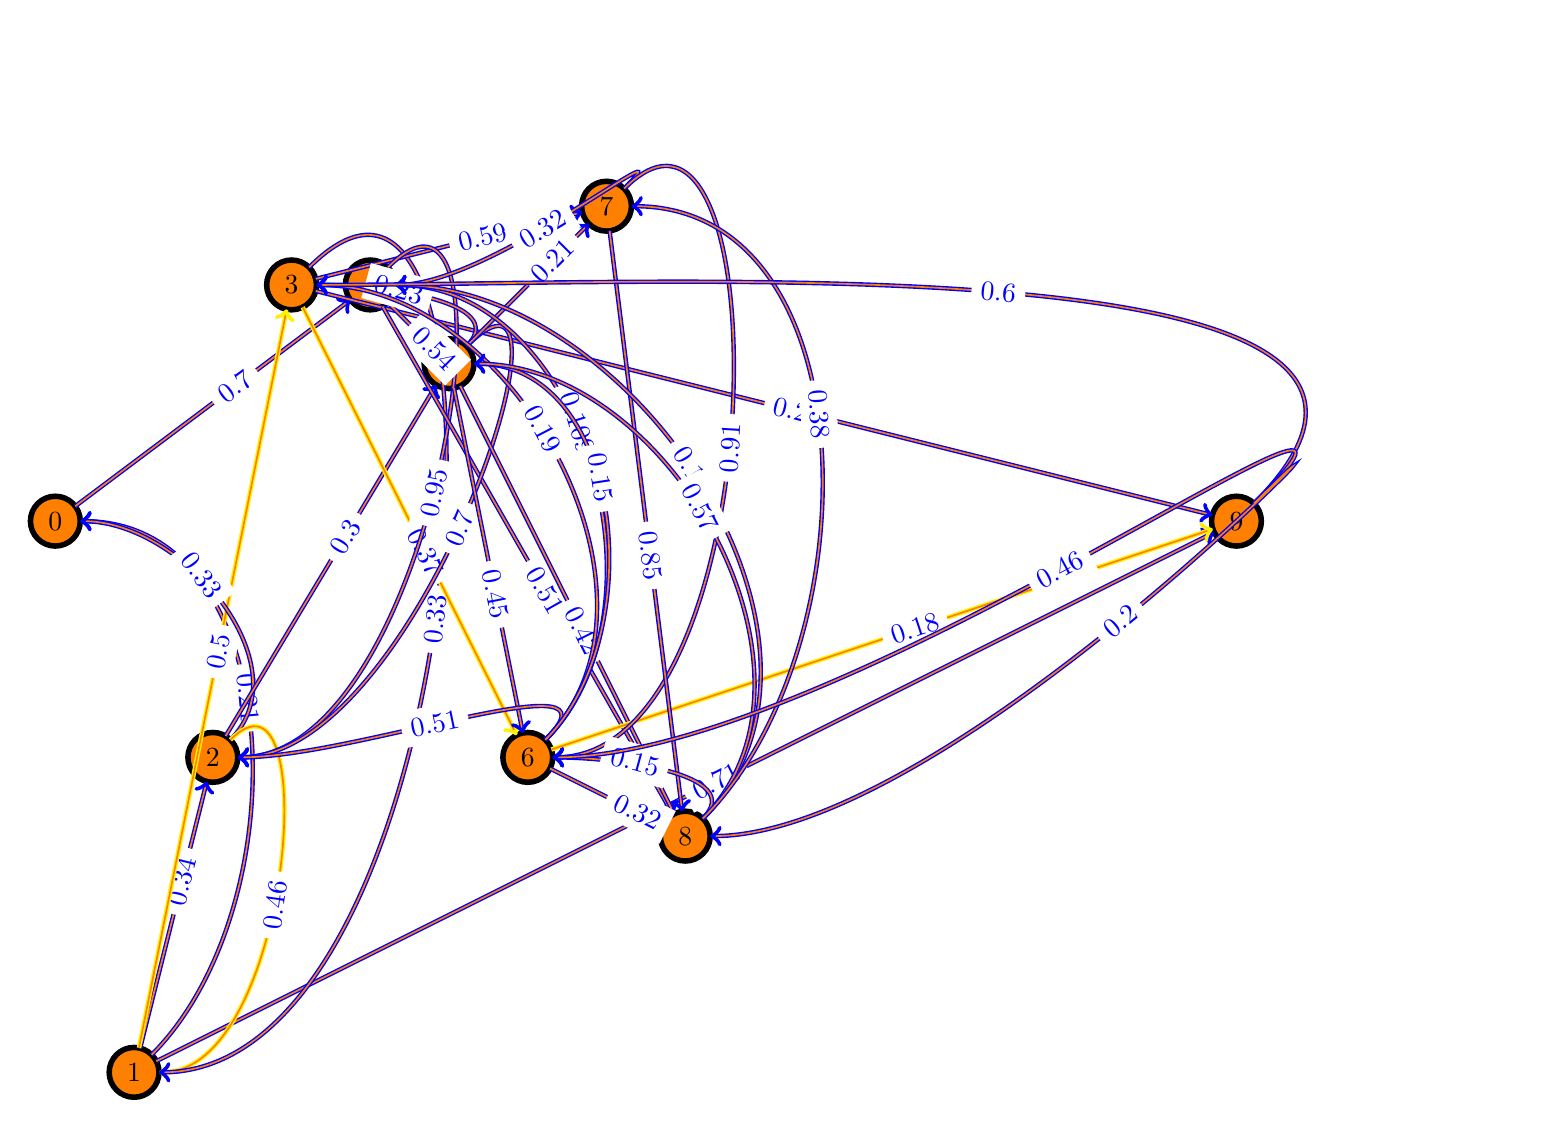
\begin{tikzpicture}
\SetVertexNormal[Shape      = circle,
FillColor  = orange,
LineWidth  = 2pt]
\SetUpEdge[lw         = 0.5pt,
color      = black,
labelcolor = white,
labeltext  = red,
labelstyle = {sloped,text=blue}]
\tikzstyle{TempStyle}=[double = orange]
\Vertex[x=-10, y=8]{0}
\Vertex[x=-9, y=1]{1}
\Vertex[x=-8, y=5]{2}
\Vertex[x=-7, y=11]{3}
\Vertex[x=-6, y=11]{4}
\Vertex[x=-5, y=10]{5}
\Vertex[x=-4, y=5]{6}
\Vertex[x=-3, y=12]{7}
\Vertex[x=-2, y=4]{8}
\Vertex[x=5, y=8]{9}
\tikzset{EdgeStyle/.style={->,TempStyle,relative=false,right=60,color=blue}}
\Edge[label=$0.7$](0)(4)
\tikzset{EdgeStyle/.style={->,TempStyle,relative=false,left=60,color=blue,in=0,draw}}
\Edge[label=$0.21$](1)(0)
\tikzset{EdgeStyle/.style={->,TempStyle,relative=false,right=60,color=blue}}
\Edge[label=$0.34$](1)(2)
\tikzset{EdgeStyle/.style={->,TempStyle,relative=false,right=60,color=yellow}}
\Edge[label=$0.5$](1)(3)
\tikzset{EdgeStyle/.style={->,TempStyle,relative=false,right=60,color=blue}}
\Edge[label=$0.71$](1)(9)
\tikzset{EdgeStyle/.style={->,TempStyle,relative=false,left=60,color=blue,in=0,draw}}
\Edge[label=$0.33$](2)(0)
\tikzset{EdgeStyle/.style={->,TempStyle,relative=false,left=60,in=0,color=yellow}}
\Edge[label=$0.46$](2)(1)
\tikzset{EdgeStyle/.style={->,TempStyle,relative=false,right=60,color=blue}}
\Edge[label=$0.3$](2)(5)
\tikzset{EdgeStyle/.style={->,TempStyle,relative=false,left=60,color=blue,in=0,draw}}
\Edge[label=$0.33$](3)(1)
\tikzset{EdgeStyle/.style={->,TempStyle,relative=false,right=60,color=yellow}}
\Edge[label=$0.37$](3)(6)
\tikzset{EdgeStyle/.style={->,TempStyle,relative=false,right=60,color=blue}}
\Edge[label=$0.59$](3)(7)
\tikzset{EdgeStyle/.style={->,TempStyle,relative=false,right=60,color=blue}}
\Edge[label=$0.2$](3)(9)
\tikzset{EdgeStyle/.style={->,TempStyle,relative=false,left=60,color=blue,in=0,draw}}
\Edge[label=$0.95$](4)(2)
\tikzset{EdgeStyle/.style={->,TempStyle,relative=false,right=60,color=blue}}
\Edge[label=$0.54$](4)(5)
\tikzset{EdgeStyle/.style={->,TempStyle,relative=false,right=60,color=blue}}
\Edge[label=$0.51$](4)(8)
\tikzset{EdgeStyle/.style={->,TempStyle,relative=false,left=60,color=blue,in=0,draw}}
\Edge[label=$0.7$](5)(2)
\tikzset{EdgeStyle/.style={->,TempStyle,relative=false,left=60,color=blue,in=0,draw}}
\Edge[label=$0.23$](5)(3)
\tikzset{EdgeStyle/.style={->,TempStyle,relative=false,right=60,color=blue}}
\Edge[label=$0.45$](5)(6)
\tikzset{EdgeStyle/.style={->,TempStyle,relative=false,right=60,color=blue}}
\Edge[label=$0.21$](5)(7)
\tikzset{EdgeStyle/.style={->,TempStyle,relative=false,right=60,color=blue}}
\Edge[label=$0.42$](5)(8)
\tikzset{EdgeStyle/.style={->,TempStyle,relative=false,left=60,color=blue,in=0,draw}}
\Edge[label=$0.51$](6)(2)
\tikzset{EdgeStyle/.style={->,TempStyle,relative=false,left=60,color=blue,in=0,draw}}
\Edge[label=$0.19$](6)(3)
\tikzset{EdgeStyle/.style={->,TempStyle,relative=false,left=60,color=blue,in=0,draw}}
\Edge[label=$0.109$](6)(4)
\tikzset{EdgeStyle/.style={->,TempStyle,relative=false,left=60,color=blue,in=0,draw}}
\Edge[label=$0.15$](6)(5)
\tikzset{EdgeStyle/.style={->,TempStyle,relative=false,right=60,color=blue}}
\Edge[label=$0.32$](6)(8)
\tikzset{EdgeStyle/.style={->,TempStyle,relative=false,right=60,color=yellow}}
\Edge[label=$0.18$](6)(9)
\tikzset{EdgeStyle/.style={->,TempStyle,relative=false,left=60,color=blue,in=0,draw}}
\Edge[label=$0.32$](7)(4)
\tikzset{EdgeStyle/.style={->,TempStyle,relative=false,left=60,color=blue,in=0,draw}}
\Edge[label=$0.91$](7)(6)
\tikzset{EdgeStyle/.style={->,TempStyle,relative=false,right=60,color=blue}}
\Edge[label=$0.85$](7)(8)
\tikzset{EdgeStyle/.style={->,TempStyle,relative=false,left=60,color=blue,in=0,draw}}
\Edge[label=$0.1$](8)(4)
\tikzset{EdgeStyle/.style={->,TempStyle,relative=false,left=60,color=blue,in=0,draw}}
\Edge[label=$0.57$](8)(5)
\tikzset{EdgeStyle/.style={->,TempStyle,relative=false,left=60,color=blue,in=0,draw}}
\Edge[label=$0.15$](8)(6)
\tikzset{EdgeStyle/.style={->,TempStyle,relative=false,left=60,color=blue,in=0,draw}}
\Edge[label=$0.38$](8)(7)
\tikzset{EdgeStyle/.style={->,TempStyle,relative=false,left=60,color=blue,in=0,draw}}
\Edge[label=$0.6$](9)(3)
\tikzset{EdgeStyle/.style={->,TempStyle,relative=false,left=60,color=blue,in=0,draw}}
\Edge[label=$0.46$](9)(6)
\tikzset{EdgeStyle/.style={->,TempStyle,relative=false,left=60,color=blue,in=0,draw}}
\Edge[label=$0.2$](9)(8)
\end{tikzpicture}\\
\begin{center}\begin{tabular}{l c}\\
\textcolor{orange}{\LARGE$\rightarrow$} & Chemin \\
 \textcolor{red}{\LARGE$\rightarrow$} & Créations arcs\\
 \textcolor{green}{\LARGE$\rightarrow$} & Modification flot\\
\end{tabular}
\end{center}
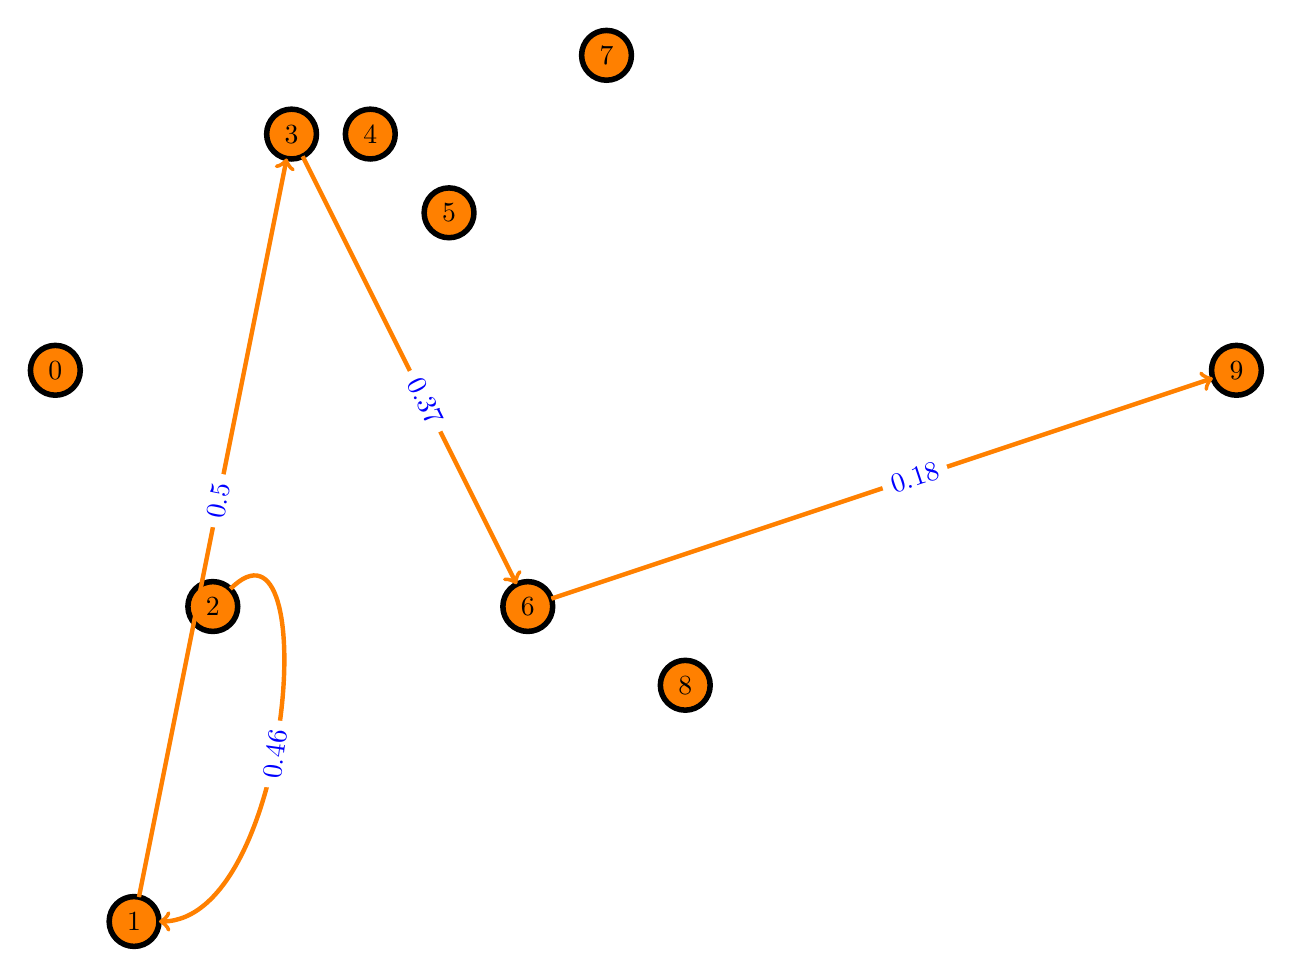
\begin{tikzpicture}
\SetVertexNormal[Shape      = circle,
FillColor  = orange,
LineWidth  = 2pt]
\SetUpEdge[lw         = 0.5pt,
color      = black,
labelcolor = white,
labeltext  = red,
labelstyle = {sloped,text=blue}]
\tikzstyle{TempStyle}=[double = orange]
\Vertex[x=-10, y=8]{0}
\Vertex[x=-9, y=1]{1}
\Vertex[x=-8, y=5]{2}
\Vertex[x=-7, y=11]{3}
\Vertex[x=-6, y=11]{4}
\Vertex[x=-5, y=10]{5}
\Vertex[x=-4, y=5]{6}
\Vertex[x=-3, y=12]{7}
\Vertex[x=-2, y=4]{8}
\Vertex[x=5, y=8]{9}
\tikzset{EdgeStyle/.style={->,TempStyle,relative=false,right=60,color=orange}}
\Edge[label=$0.5$](1)(3)
\tikzset{EdgeStyle/.style={->,TempStyle,relative=false,left=60,color=orange,in=0,draw}}
\Edge[label=$0.46$](2)(1)
\tikzset{EdgeStyle/.style={->,TempStyle,relative=false,right=60,color=orange}}
\Edge[label=$0.37$](3)(6)
\tikzset{EdgeStyle/.style={->,TempStyle,relative=false,right=60,color=orange}}
\Edge[label=$0.18$](6)(9)
\end{tikzpicture}\\
\begin{center}\begin{tabular}{l c}\\
\textcolor{orange}{\LARGE$\rightarrow$} & Chemin \\
 \textcolor{red}{\LARGE$\rightarrow$} & Créations arcs\\
 \textcolor{green}{\LARGE$\rightarrow$} & Modification flot\\
\end{tabular}
\end{center}
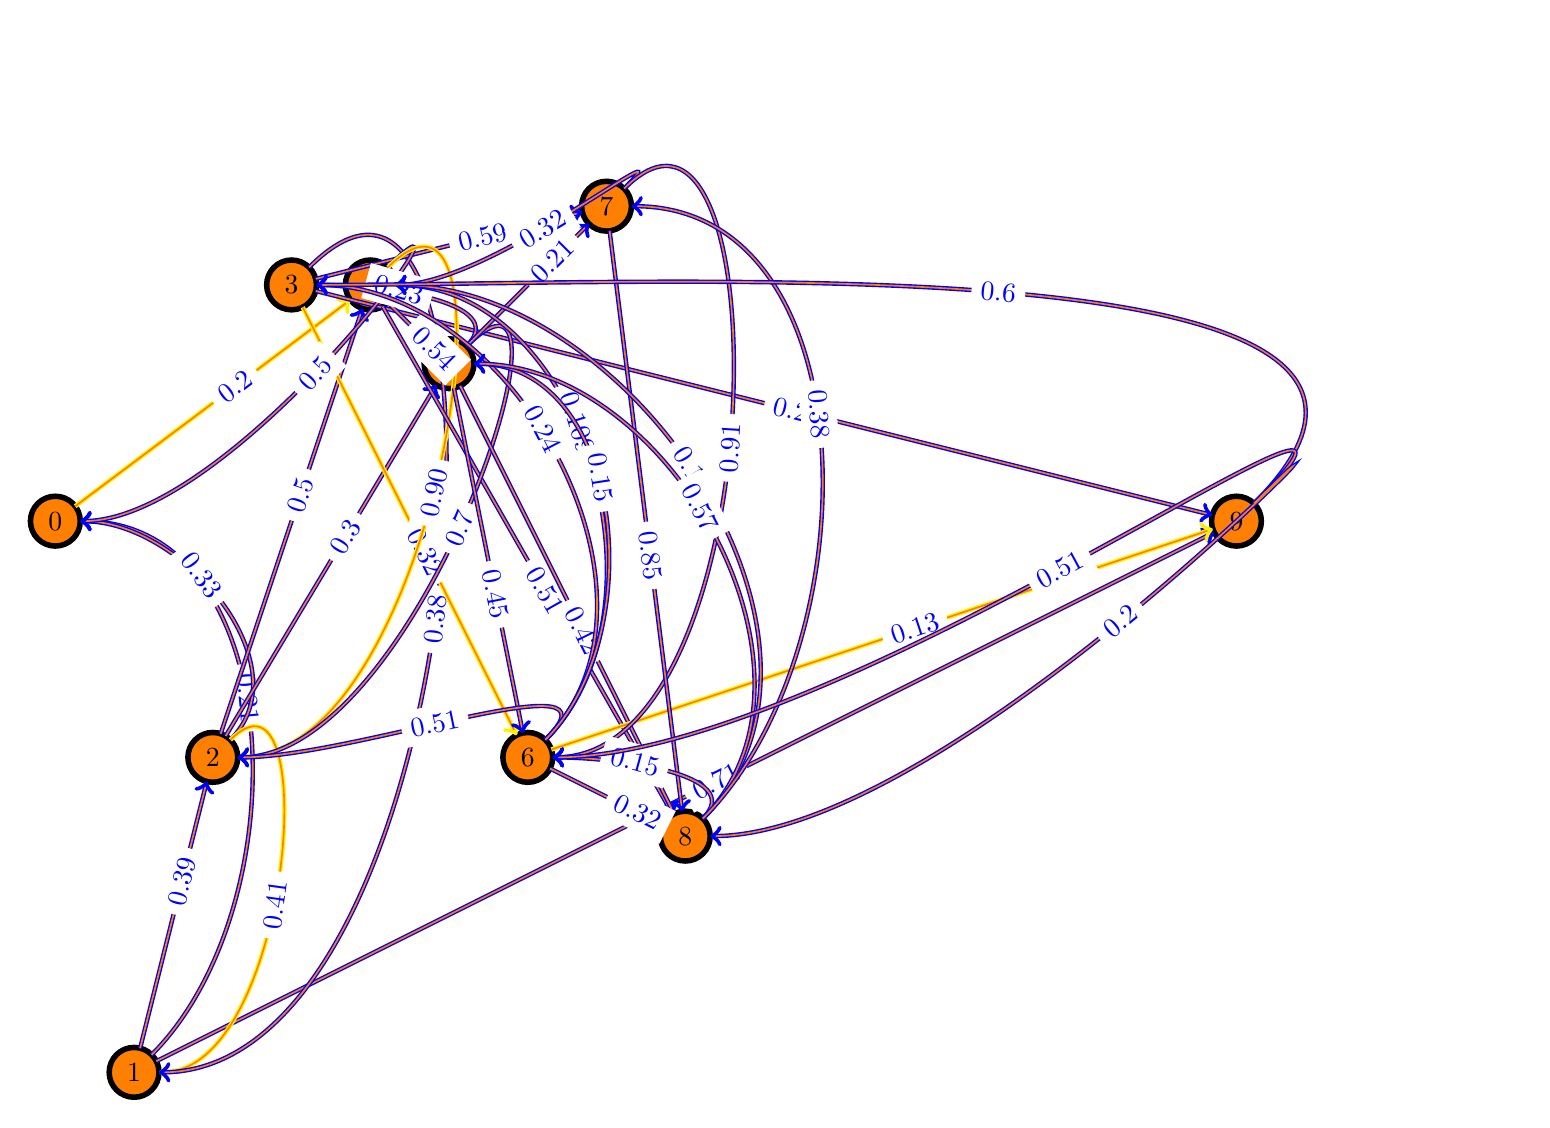
\begin{tikzpicture}
\SetVertexNormal[Shape      = circle,
FillColor  = orange,
LineWidth  = 2pt]
\SetUpEdge[lw         = 0.5pt,
color      = black,
labelcolor = white,
labeltext  = red,
labelstyle = {sloped,text=blue}]
\tikzstyle{TempStyle}=[double = orange]
\Vertex[x=-10, y=8]{0}
\Vertex[x=-9, y=1]{1}
\Vertex[x=-8, y=5]{2}
\Vertex[x=-7, y=11]{3}
\Vertex[x=-6, y=11]{4}
\Vertex[x=-5, y=10]{5}
\Vertex[x=-4, y=5]{6}
\Vertex[x=-3, y=12]{7}
\Vertex[x=-2, y=4]{8}
\Vertex[x=5, y=8]{9}
\tikzset{EdgeStyle/.style={->,TempStyle,relative=false,right=60,color=yellow}}
\Edge[label=$0.2$](0)(4)
\tikzset{EdgeStyle/.style={->,TempStyle,relative=false,left=60,color=blue,in=0,draw}}
\Edge[label=$0.21$](1)(0)
\tikzset{EdgeStyle/.style={->,TempStyle,relative=false,right=60,color=blue}}
\Edge[label=$0.39$](1)(2)
\tikzset{EdgeStyle/.style={->,TempStyle,relative=false,right=60,color=blue}}
\Edge[label=$0.71$](1)(9)
\tikzset{EdgeStyle/.style={->,TempStyle,relative=false,left=60,color=blue,in=0,draw}}
\Edge[label=$0.33$](2)(0)
\tikzset{EdgeStyle/.style={->,TempStyle,relative=false,left=60,in=0,color=yellow}}
\Edge[label=$0.41$](2)(1)
\tikzset{EdgeStyle/.style={->,TempStyle,relative=false,right=60,color=blue}}
\Edge[label=$0.5$](2)(4)
\tikzset{EdgeStyle/.style={->,TempStyle,relative=false,right=60,color=blue}}
\Edge[label=$0.3$](2)(5)
\tikzset{EdgeStyle/.style={->,TempStyle,relative=false,left=60,color=blue,in=0,draw}}
\Edge[label=$0.38$](3)(1)
\tikzset{EdgeStyle/.style={->,TempStyle,relative=false,right=60,color=yellow}}
\Edge[label=$0.32$](3)(6)
\tikzset{EdgeStyle/.style={->,TempStyle,relative=false,right=60,color=blue}}
\Edge[label=$0.59$](3)(7)
\tikzset{EdgeStyle/.style={->,TempStyle,relative=false,right=60,color=blue}}
\Edge[label=$0.2$](3)(9)
\tikzset{EdgeStyle/.style={->,TempStyle,relative=false,left=60,color=blue,in=0,draw}}
\Edge[label=$0.5$](4)(0)
\tikzset{EdgeStyle/.style={->,TempStyle,relative=false,left=60,in=0,color=yellow}}
\Edge[label=$0.90$](4)(2)
\tikzset{EdgeStyle/.style={->,TempStyle,relative=false,right=60,color=blue}}
\Edge[label=$0.54$](4)(5)
\tikzset{EdgeStyle/.style={->,TempStyle,relative=false,right=60,color=blue}}
\Edge[label=$0.51$](4)(8)
\tikzset{EdgeStyle/.style={->,TempStyle,relative=false,left=60,color=blue,in=0,draw}}
\Edge[label=$0.7$](5)(2)
\tikzset{EdgeStyle/.style={->,TempStyle,relative=false,left=60,color=blue,in=0,draw}}
\Edge[label=$0.23$](5)(3)
\tikzset{EdgeStyle/.style={->,TempStyle,relative=false,right=60,color=blue}}
\Edge[label=$0.45$](5)(6)
\tikzset{EdgeStyle/.style={->,TempStyle,relative=false,right=60,color=blue}}
\Edge[label=$0.21$](5)(7)
\tikzset{EdgeStyle/.style={->,TempStyle,relative=false,right=60,color=blue}}
\Edge[label=$0.42$](5)(8)
\tikzset{EdgeStyle/.style={->,TempStyle,relative=false,left=60,color=blue,in=0,draw}}
\Edge[label=$0.51$](6)(2)
\tikzset{EdgeStyle/.style={->,TempStyle,relative=false,left=60,color=blue,in=0,draw}}
\Edge[label=$0.24$](6)(3)
\tikzset{EdgeStyle/.style={->,TempStyle,relative=false,left=60,color=blue,in=0,draw}}
\Edge[label=$0.109$](6)(4)
\tikzset{EdgeStyle/.style={->,TempStyle,relative=false,left=60,color=blue,in=0,draw}}
\Edge[label=$0.15$](6)(5)
\tikzset{EdgeStyle/.style={->,TempStyle,relative=false,right=60,color=blue}}
\Edge[label=$0.32$](6)(8)
\tikzset{EdgeStyle/.style={->,TempStyle,relative=false,right=60,color=yellow}}
\Edge[label=$0.13$](6)(9)
\tikzset{EdgeStyle/.style={->,TempStyle,relative=false,left=60,color=blue,in=0,draw}}
\Edge[label=$0.32$](7)(4)
\tikzset{EdgeStyle/.style={->,TempStyle,relative=false,left=60,color=blue,in=0,draw}}
\Edge[label=$0.91$](7)(6)
\tikzset{EdgeStyle/.style={->,TempStyle,relative=false,right=60,color=blue}}
\Edge[label=$0.85$](7)(8)
\tikzset{EdgeStyle/.style={->,TempStyle,relative=false,left=60,color=blue,in=0,draw}}
\Edge[label=$0.1$](8)(4)
\tikzset{EdgeStyle/.style={->,TempStyle,relative=false,left=60,color=blue,in=0,draw}}
\Edge[label=$0.57$](8)(5)
\tikzset{EdgeStyle/.style={->,TempStyle,relative=false,left=60,color=blue,in=0,draw}}
\Edge[label=$0.15$](8)(6)
\tikzset{EdgeStyle/.style={->,TempStyle,relative=false,left=60,color=blue,in=0,draw}}
\Edge[label=$0.38$](8)(7)
\tikzset{EdgeStyle/.style={->,TempStyle,relative=false,left=60,color=blue,in=0,draw}}
\Edge[label=$0.6$](9)(3)
\tikzset{EdgeStyle/.style={->,TempStyle,relative=false,left=60,color=blue,in=0,draw}}
\Edge[label=$0.51$](9)(6)
\tikzset{EdgeStyle/.style={->,TempStyle,relative=false,left=60,color=blue,in=0,draw}}
\Edge[label=$0.2$](9)(8)
\end{tikzpicture}\\
\begin{center}\begin{tabular}{l c}\\
\textcolor{orange}{\LARGE$\rightarrow$} & Chemin \\
 \textcolor{red}{\LARGE$\rightarrow$} & Créations arcs\\
 \textcolor{green}{\LARGE$\rightarrow$} & Modification flot\\
\end{tabular}
\end{center}
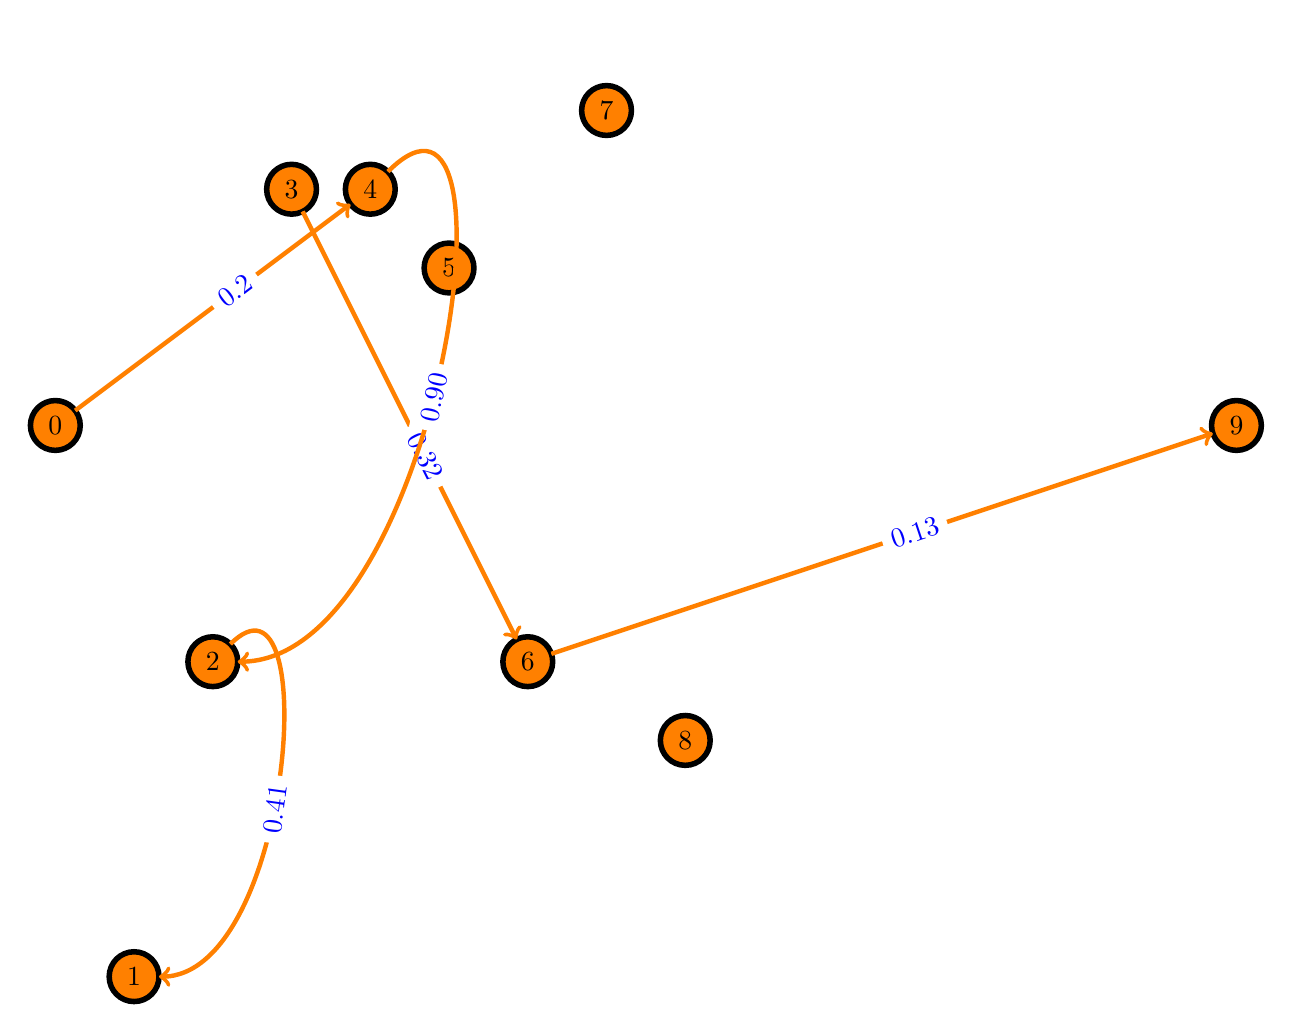
\begin{tikzpicture}
\SetVertexNormal[Shape      = circle,
FillColor  = orange,
LineWidth  = 2pt]
\SetUpEdge[lw         = 0.5pt,
color      = black,
labelcolor = white,
labeltext  = red,
labelstyle = {sloped,text=blue}]
\tikzstyle{TempStyle}=[double = orange]
\Vertex[x=-10, y=8]{0}
\Vertex[x=-9, y=1]{1}
\Vertex[x=-8, y=5]{2}
\Vertex[x=-7, y=11]{3}
\Vertex[x=-6, y=11]{4}
\Vertex[x=-5, y=10]{5}
\Vertex[x=-4, y=5]{6}
\Vertex[x=-3, y=12]{7}
\Vertex[x=-2, y=4]{8}
\Vertex[x=5, y=8]{9}
\tikzset{EdgeStyle/.style={->,TempStyle,relative=false,right=60,color=orange}}
\Edge[label=$0.2$](0)(4)
\tikzset{EdgeStyle/.style={->,TempStyle,relative=false,left=60,color=orange,in=0,draw}}
\Edge[label=$0.41$](2)(1)
\tikzset{EdgeStyle/.style={->,TempStyle,relative=false,right=60,color=orange}}
\Edge[label=$0.32$](3)(6)
\tikzset{EdgeStyle/.style={->,TempStyle,relative=false,left=60,color=orange,in=0,draw}}
\Edge[label=$0.90$](4)(2)
\tikzset{EdgeStyle/.style={->,TempStyle,relative=false,right=60,color=orange}}
\Edge[label=$0.13$](6)(9)
\end{tikzpicture}\\
\begin{center}\begin{tabular}{l c}\\
\textcolor{orange}{\LARGE$\rightarrow$} & Chemin \\
 \textcolor{red}{\LARGE$\rightarrow$} & Créations arcs\\
 \textcolor{green}{\LARGE$\rightarrow$} & Modification flot\\
\end{tabular}
\end{center}
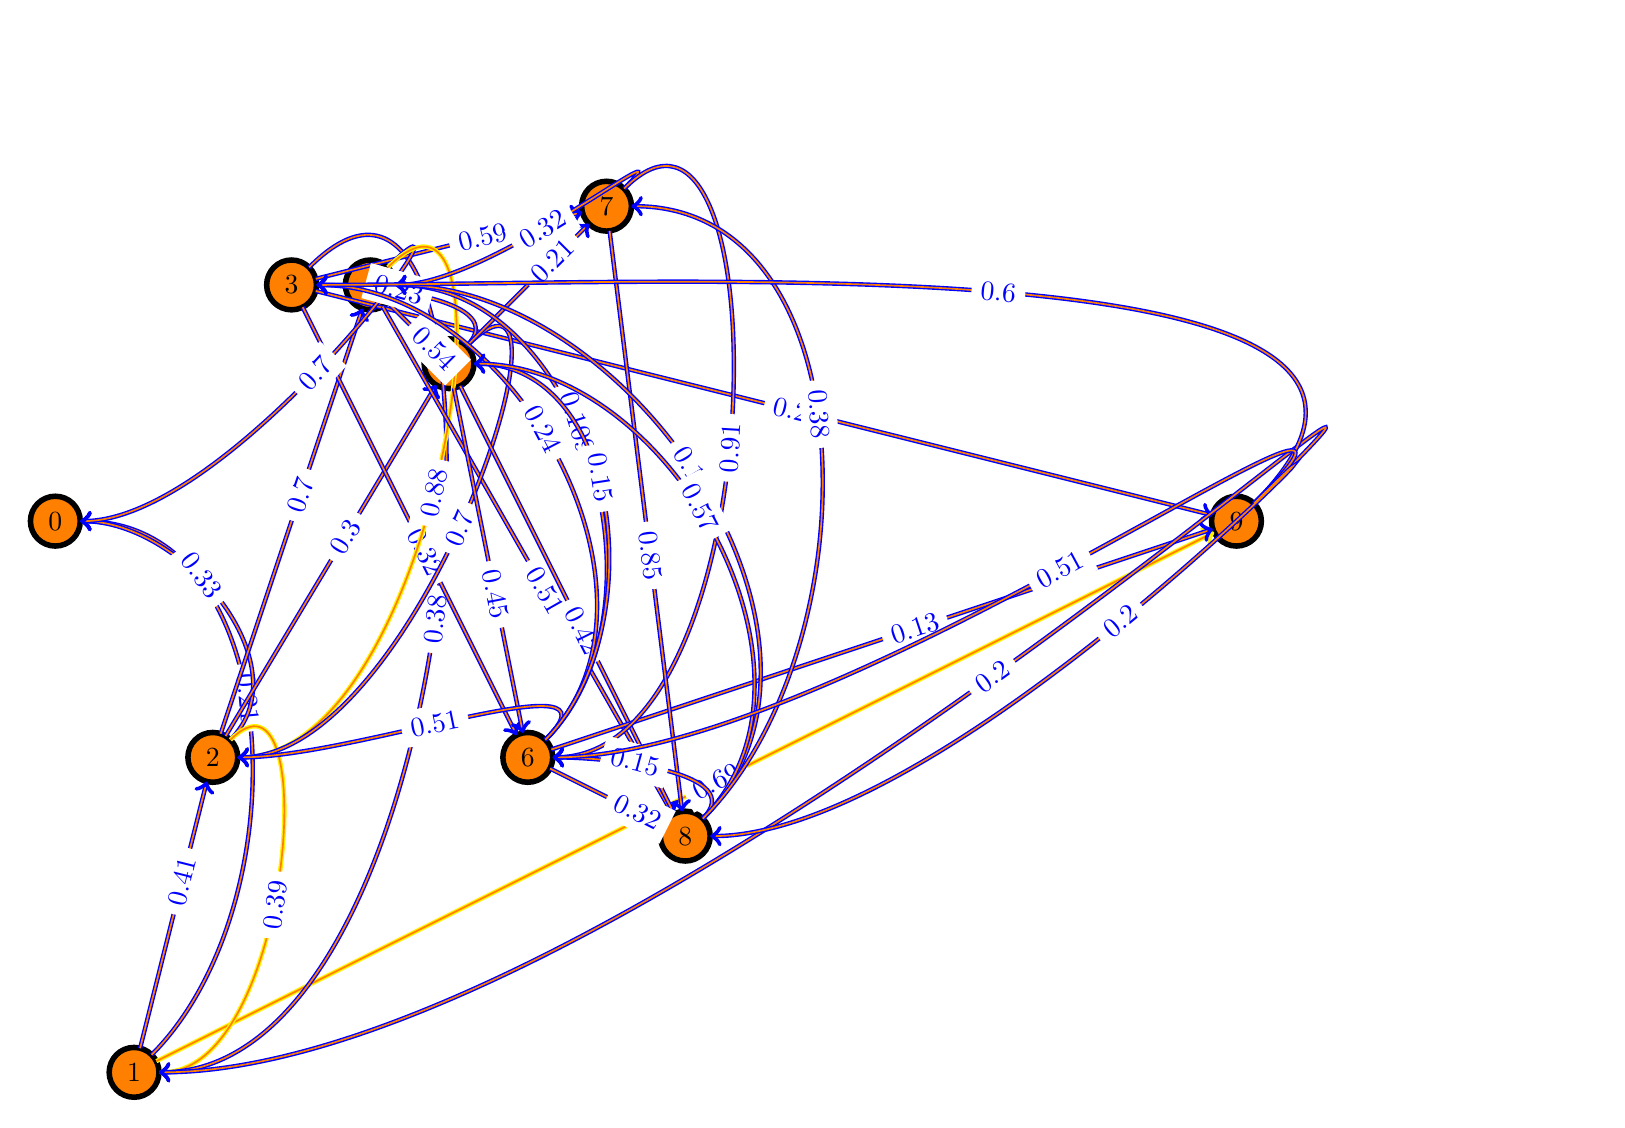
\begin{tikzpicture}
\SetVertexNormal[Shape      = circle,
FillColor  = orange,
LineWidth  = 2pt]
\SetUpEdge[lw         = 0.5pt,
color      = black,
labelcolor = white,
labeltext  = red,
labelstyle = {sloped,text=blue}]
\tikzstyle{TempStyle}=[double = orange]
\Vertex[x=-10, y=8]{0}
\Vertex[x=-9, y=1]{1}
\Vertex[x=-8, y=5]{2}
\Vertex[x=-7, y=11]{3}
\Vertex[x=-6, y=11]{4}
\Vertex[x=-5, y=10]{5}
\Vertex[x=-4, y=5]{6}
\Vertex[x=-3, y=12]{7}
\Vertex[x=-2, y=4]{8}
\Vertex[x=5, y=8]{9}
\tikzset{EdgeStyle/.style={->,TempStyle,relative=false,left=60,color=blue,in=0,draw}}
\Edge[label=$0.21$](1)(0)
\tikzset{EdgeStyle/.style={->,TempStyle,relative=false,right=60,color=blue}}
\Edge[label=$0.41$](1)(2)
\tikzset{EdgeStyle/.style={->,TempStyle,relative=false,right=60,color=yellow}}
\Edge[label=$0.69$](1)(9)
\tikzset{EdgeStyle/.style={->,TempStyle,relative=false,left=60,color=blue,in=0,draw}}
\Edge[label=$0.33$](2)(0)
\tikzset{EdgeStyle/.style={->,TempStyle,relative=false,left=60,in=0,color=yellow}}
\Edge[label=$0.39$](2)(1)
\tikzset{EdgeStyle/.style={->,TempStyle,relative=false,right=60,color=blue}}
\Edge[label=$0.7$](2)(4)
\tikzset{EdgeStyle/.style={->,TempStyle,relative=false,right=60,color=blue}}
\Edge[label=$0.3$](2)(5)
\tikzset{EdgeStyle/.style={->,TempStyle,relative=false,left=60,color=blue,in=0,draw}}
\Edge[label=$0.38$](3)(1)
\tikzset{EdgeStyle/.style={->,TempStyle,relative=false,right=60,color=blue}}
\Edge[label=$0.32$](3)(6)
\tikzset{EdgeStyle/.style={->,TempStyle,relative=false,right=60,color=blue}}
\Edge[label=$0.59$](3)(7)
\tikzset{EdgeStyle/.style={->,TempStyle,relative=false,right=60,color=blue}}
\Edge[label=$0.2$](3)(9)
\tikzset{EdgeStyle/.style={->,TempStyle,relative=false,left=60,color=blue,in=0,draw}}
\Edge[label=$0.7$](4)(0)
\tikzset{EdgeStyle/.style={->,TempStyle,relative=false,left=60,in=0,color=yellow}}
\Edge[label=$0.88$](4)(2)
\tikzset{EdgeStyle/.style={->,TempStyle,relative=false,right=60,color=blue}}
\Edge[label=$0.54$](4)(5)
\tikzset{EdgeStyle/.style={->,TempStyle,relative=false,right=60,color=blue}}
\Edge[label=$0.51$](4)(8)
\tikzset{EdgeStyle/.style={->,TempStyle,relative=false,left=60,color=blue,in=0,draw}}
\Edge[label=$0.7$](5)(2)
\tikzset{EdgeStyle/.style={->,TempStyle,relative=false,left=60,color=blue,in=0,draw}}
\Edge[label=$0.23$](5)(3)
\tikzset{EdgeStyle/.style={->,TempStyle,relative=false,right=60,color=blue}}
\Edge[label=$0.45$](5)(6)
\tikzset{EdgeStyle/.style={->,TempStyle,relative=false,right=60,color=blue}}
\Edge[label=$0.21$](5)(7)
\tikzset{EdgeStyle/.style={->,TempStyle,relative=false,right=60,color=blue}}
\Edge[label=$0.42$](5)(8)
\tikzset{EdgeStyle/.style={->,TempStyle,relative=false,left=60,color=blue,in=0,draw}}
\Edge[label=$0.51$](6)(2)
\tikzset{EdgeStyle/.style={->,TempStyle,relative=false,left=60,color=blue,in=0,draw}}
\Edge[label=$0.24$](6)(3)
\tikzset{EdgeStyle/.style={->,TempStyle,relative=false,left=60,color=blue,in=0,draw}}
\Edge[label=$0.109$](6)(4)
\tikzset{EdgeStyle/.style={->,TempStyle,relative=false,left=60,color=blue,in=0,draw}}
\Edge[label=$0.15$](6)(5)
\tikzset{EdgeStyle/.style={->,TempStyle,relative=false,right=60,color=blue}}
\Edge[label=$0.32$](6)(8)
\tikzset{EdgeStyle/.style={->,TempStyle,relative=false,right=60,color=blue}}
\Edge[label=$0.13$](6)(9)
\tikzset{EdgeStyle/.style={->,TempStyle,relative=false,left=60,color=blue,in=0,draw}}
\Edge[label=$0.32$](7)(4)
\tikzset{EdgeStyle/.style={->,TempStyle,relative=false,left=60,color=blue,in=0,draw}}
\Edge[label=$0.91$](7)(6)
\tikzset{EdgeStyle/.style={->,TempStyle,relative=false,right=60,color=blue}}
\Edge[label=$0.85$](7)(8)
\tikzset{EdgeStyle/.style={->,TempStyle,relative=false,left=60,color=blue,in=0,draw}}
\Edge[label=$0.1$](8)(4)
\tikzset{EdgeStyle/.style={->,TempStyle,relative=false,left=60,color=blue,in=0,draw}}
\Edge[label=$0.57$](8)(5)
\tikzset{EdgeStyle/.style={->,TempStyle,relative=false,left=60,color=blue,in=0,draw}}
\Edge[label=$0.15$](8)(6)
\tikzset{EdgeStyle/.style={->,TempStyle,relative=false,left=60,color=blue,in=0,draw}}
\Edge[label=$0.38$](8)(7)
\tikzset{EdgeStyle/.style={->,TempStyle,relative=false,left=60,color=blue,in=0,draw}}
\Edge[label=$0.2$](9)(1)
\tikzset{EdgeStyle/.style={->,TempStyle,relative=false,left=60,color=blue,in=0,draw}}
\Edge[label=$0.6$](9)(3)
\tikzset{EdgeStyle/.style={->,TempStyle,relative=false,left=60,color=blue,in=0,draw}}
\Edge[label=$0.51$](9)(6)
\tikzset{EdgeStyle/.style={->,TempStyle,relative=false,left=60,color=blue,in=0,draw}}
\Edge[label=$0.2$](9)(8)
\end{tikzpicture}\\
\begin{center}\begin{tabular}{l c}\\
\textcolor{orange}{\LARGE$\rightarrow$} & Chemin \\
 \textcolor{red}{\LARGE$\rightarrow$} & Créations arcs\\
 \textcolor{green}{\LARGE$\rightarrow$} & Modification flot\\
\end{tabular}
\end{center}
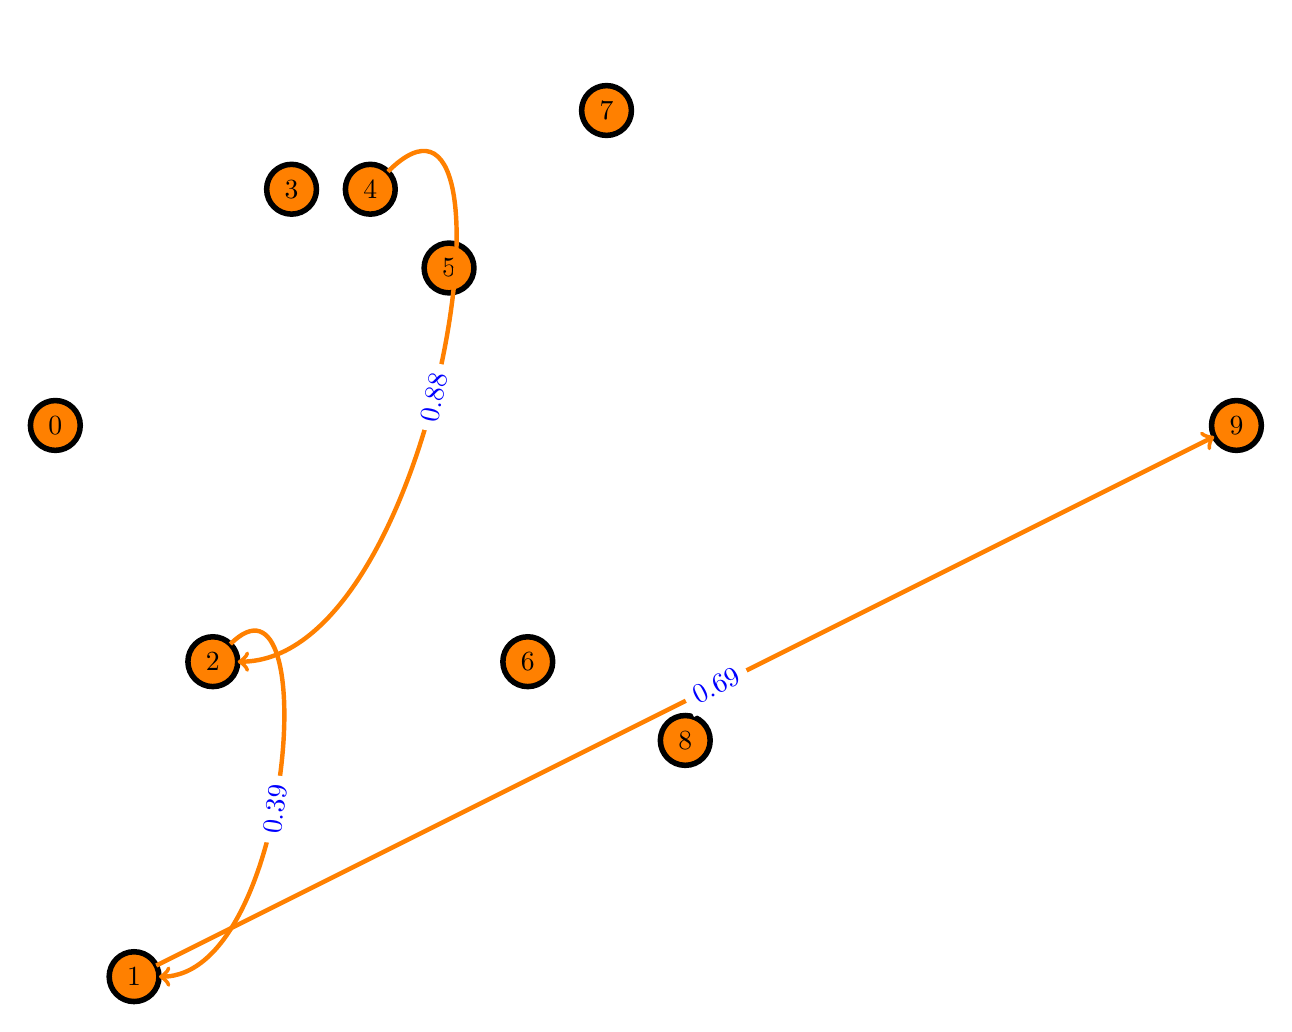
\begin{tikzpicture}
\SetVertexNormal[Shape      = circle,
FillColor  = orange,
LineWidth  = 2pt]
\SetUpEdge[lw         = 0.5pt,
color      = black,
labelcolor = white,
labeltext  = red,
labelstyle = {sloped,text=blue}]
\tikzstyle{TempStyle}=[double = orange]
\Vertex[x=-10, y=8]{0}
\Vertex[x=-9, y=1]{1}
\Vertex[x=-8, y=5]{2}
\Vertex[x=-7, y=11]{3}
\Vertex[x=-6, y=11]{4}
\Vertex[x=-5, y=10]{5}
\Vertex[x=-4, y=5]{6}
\Vertex[x=-3, y=12]{7}
\Vertex[x=-2, y=4]{8}
\Vertex[x=5, y=8]{9}
\tikzset{EdgeStyle/.style={->,TempStyle,relative=false,right=60,color=orange}}
\Edge[label=$0.69$](1)(9)
\tikzset{EdgeStyle/.style={->,TempStyle,relative=false,left=60,color=orange,in=0,draw}}
\Edge[label=$0.39$](2)(1)
\tikzset{EdgeStyle/.style={->,TempStyle,relative=false,left=60,color=orange,in=0,draw}}
\Edge[label=$0.88$](4)(2)
\end{tikzpicture}\\
\begin{center}\begin{tabular}{l c}\\
\textcolor{orange}{\LARGE$\rightarrow$} & Chemin \\
 \textcolor{red}{\LARGE$\rightarrow$} & Créations arcs\\
 \textcolor{green}{\LARGE$\rightarrow$} & Modification flot\\
\end{tabular}
\end{center}
\end{document}
